\documentclass[11pt,a4paper,fontset=none]{ctexart}
\setCJKmainfont{Noto Serif CJK SC}[BoldFont={Noto Sans CJK SC Bold}]
\setCJKsansfont{Noto Sans CJK SC}
\setCJKmonofont{Noto Sans CJK SC}
\usepackage[margin=2.3cm]{geometry}
\usepackage{amsmath,amssymb}
\usepackage{booktabs,multirow}
\usepackage{graphicx}
\usepackage{float}
\usepackage{caption}
\usepackage{enumitem}
\usepackage{algorithm}
\usepackage{algpseudocode}
\usepackage{tikz}
\usetikzlibrary{arrows.meta,positioning,calc}
\usepackage{cite}
\usepackage[hidelinks]{hyperref}
\graphicspath{{../results/}}
\setlist{itemsep=2pt,topsep=4pt}
\newcommand{\code}[1]{\texttt{#1}}
\newcommand{\pct}{\,\%}
% 表格行由 report/case_study.py 生成（原语 input 可在 tabular 内使用）。
\makeatletter\newcommand{\inputrows}[1]{\@@input #1 }\makeatother
\floatname{algorithm}{算法}
\renewcommand{\algorithmicwhile}{\textbf{当}}
\renewcommand{\algorithmicdo}{\textbf{执行}}
\algrenewtext{EndWhile}{\textbf{结束循环}}

\title{双环路配送机器人交叉口通行与\\共享充电资源联合调度}
\author{EE6228 课程项目（M02 与 M04 联合选题）}
\date{纯软件二维在线仿真}

\begin{document}
\maketitle

\begin{abstract}
四台配送机器人在两条单向环路上工作，两条环路共用一个互斥交叉口，并共用一个只能经由该交叉口到达的充电区。
本项目构建了确定性离散事件仿真器、独立的调度验证器和浏览器回放界面，定义了归一化目标函数，并比较了四种启发式规则、
一个同时决定任务分配、任务顺序、交叉口时隙、充电位选择和充电量的离线 CP-SAT 模型，以及它的在线滚动时域版本。
在 700 次通过验证的运行（10 种设置 $\times$ 10 个随机种子 $\times$ 7 种策略）中，CP-SAT 相对先到先服务（FCFS）
将目标值降低约 50\pct（迟到时间减少 62\pct，完工时间缩短 28\pct），在线滚动版本降低约 37\pct，而各单一规则基线之间
相差不过几个百分点。我们还说明：公平比较要求所有方法在时域末端保留相同的电量储备；并讨论了归一化目标函数的局限。
最后用一个 12 个任务的算例完整展示一份调度：任务分配、每次进入交叉口的时刻、每次充电操作以及电量曲线。
\end{abstract}

\section{案例介绍}

两个配送区域 A 和 B 各由一条封闭的单向环路服务。两条环路在唯一的互斥交叉口 X 相交，两个区域共用一个充电区
（入口 H，充电位 C1 和 C2），充电区只能经由 X 到达。网络中有四台虚拟机器人：R1 和 R2 服务区域 A，R3 和 R4
服务区域 B。取送任务随时间到达，每个任务有释放时间、取货站、送货站、装卸时间、截止时间和优先级。

两类共享资源相互耦合。需要充电的机器人必须两次通过 X（去和回），因此交叉口拥堵会推迟充电；充电排队反过来又会推迟该机器人
以及排在其后的机器人此后的所有交叉口请求。电池约束使问题更难：机器人只有在完成任务后仍能在不低于安全阈值的情况下到达充电位时，
才能接受该任务。本项目研究如何协调\textbf{任务分配、任务顺序、交叉口时隙、充电位选择和充电时长}，
使机器人队伍在高负载下保持安全与准时。

\emph{范围。}地图和数据均为自行设计；机器人沿固定的有向路线移动（不考虑连续运动学和避障）；电量、装卸和充电均为软件状态。
研究重点是调度与资源冲突。

\subsection{相关工作}

自动导引车（AGV）的调度、路径规划与控制已有大量综述 \cite{qiu2002,vis2006,leanh2006,ganesharajah1998,deryck2020}。
这些综述区分了每次只决定一辆车或一个任务的派车规则，以及同时决定分配、排序和无冲突时序的优化方法；本文的基线策略属于前者，
CP-SAT 属于后者。大规模仓储机器人队伍由中央集中分配任务和资源，再由各机器人自行规划路径 \cite{wurman2008}，多智能体路径规划则对图上的无碰撞移动
给出了形式化定义 \cite{stern2019}。在时空上预约交叉口（即本文 X 的预约日历所做的事）由 Dresner 和 Stone 针对自动驾驶车辆提出
\cite{dresner2008}。电池约束对 AGV 的仿真和规划有重要影响 \cite{mchaney1995,kabir2018}；在电动车辆路径问题中，充电站
\cite{schneider2014}、部分充电 \cite{keskin2016} 和非线性充电曲线 \cite{montoya2017} 都被显式建模。本文的优化器采用基于约束的
调度方法，使用可选区间变量和不重叠约束 \cite{baptiste2001,laborie2018}，由 Google OR-Tools 中的 CP-SAT 求解器求解
\cite{perron2023cpsat,ortools}；CP-SAT 以惰性子句生成 \cite{ohrimenko2009} 为基础，并在其并行线程中使用大邻域搜索
\cite{shaw1998}。在线版本采用滚动（后退）时域原理 \cite{sethi1991,mayne2000}。

\section{系统描述}

\subsection{网络}

每条环路是有向回路 $X \to Z_1 \to Z_2 \to Z_3 \to Z_4 \to W_Z \to X$，其中 $Z \in \{A, B\}$（图~\ref{fig:network}）。
$W_A$ 和 $W_B$ 是机器人等待通过交叉口的唯一位置。所有进入 X 的边（$W_A \to X$、$W_B \to X$、$H \to X$）都是一次
\emph{通过}；X 同一时刻最多容纳一台机器人，相邻两次通过之间两侧各需保留安全间隔 $\beta$。充电支路为
$X \to H \to C_p \to H \to X$；机器人在 H 排队，绝不在 X 内或已被占用的充电位内等待，充电结束后立即离开充电位。

由于机器人沿环路行驶，每绕一圈都会经过 X：交叉口不仅位于去充电的路上，也位于每个送货点在取货点“后方”的配送路径上，
以及每次绕环的空驶调度路径上。

\begin{figure}[H]
\centering
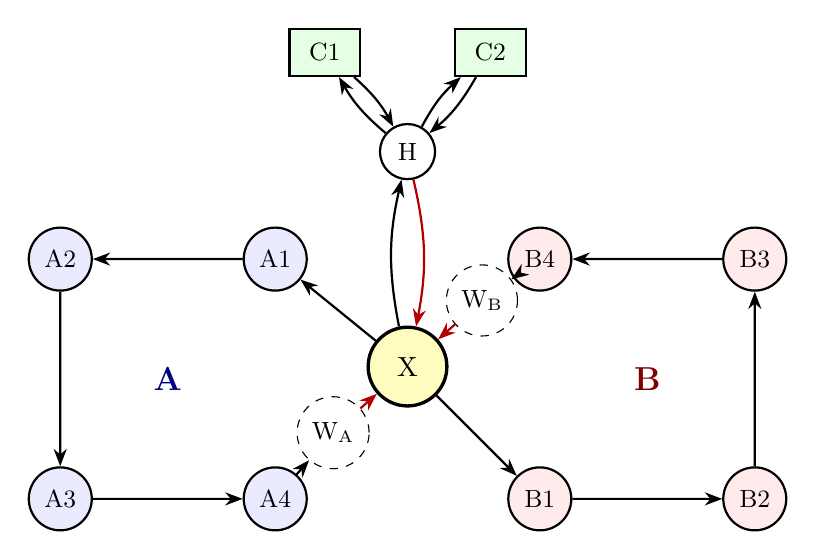
\begin{tikzpicture}[
  st/.style={circle,draw,thick,minimum size=8mm,font=\small},
  wt/.style={circle,draw,dashed,minimum size=7mm,font=\small},
  bay/.style={rectangle,draw,thick,minimum width=9mm,minimum height=6mm,font=\small},
  ed/.style={-{Stealth[length=2.2mm]},thick},
  scale=1.05]
  \node[circle,draw,very thick,fill=yellow!25,minimum size=10mm] (X) at (0,0) {X};
  \node[st,fill=blue!8] (A1) at (-1.6,1.3) {A1};
  \node[st,fill=blue!8] (A2) at (-4.2,1.3) {A2};
  \node[st,fill=blue!8] (A3) at (-4.2,-1.6) {A3};
  \node[st,fill=blue!8] (A4) at (-1.6,-1.6) {A4};
  \node[wt] (WA) at (-0.9,-0.8) {W\textsubscript{A}};
  \node[st,fill=red!8] (B1) at (1.6,-1.6) {B1};
  \node[st,fill=red!8] (B2) at (4.2,-1.6) {B2};
  \node[st,fill=red!8] (B3) at (4.2,1.3) {B3};
  \node[st,fill=red!8] (B4) at (1.6,1.3) {B4};
  \node[wt] (WB) at (0.9,0.8) {W\textsubscript{B}};
  \node[circle,draw,thick,minimum size=7mm,font=\small] (H) at (0,2.6) {H};
  \node[bay,fill=green!10] (C1) at (-1.0,3.8) {C1};
  \node[bay,fill=green!10] (C2) at (1.0,3.8) {C2};
  \draw[ed] (X) -- (A1); \draw[ed] (A1) -- (A2); \draw[ed] (A2) -- (A3);
  \draw[ed] (A3) -- (A4); \draw[ed] (A4) -- (WA); \draw[ed,red!70!black] (WA) -- (X);
  \draw[ed] (X) -- (B1); \draw[ed] (B1) -- (B2); \draw[ed] (B2) -- (B3);
  \draw[ed] (B3) -- (B4); \draw[ed] (B4) -- (WB); \draw[ed,red!70!black] (WB) -- (X);
  \draw[ed] (X) to[bend left=12] (H); \draw[ed,red!70!black] (H) to[bend left=12] (X);
  \draw[ed] (H) to[bend left=10] (C1); \draw[ed] (C1) to[bend left=10] (H);
  \draw[ed] (H) to[bend left=10] (C2); \draw[ed] (C2) to[bend left=10] (H);
  \node[font=\large\bfseries,blue!50!black] at (-2.9,-0.15) {A};
  \node[font=\large\bfseries,red!50!black] at (2.9,-0.15) {B};
\end{tikzpicture}
\caption{实际实现的网络。红色箭头表示进入互斥交叉口 X 的通过；虚线节点为 X 前的等待点。R1/R2 从 A1 出发，R3/R4 从 B1 出发。}
\label{fig:network}
\end{figure}

\subsection{默认参数}

\begin{table}[!htbp]
\centering\small
\begin{tabular}{lll}
\toprule
参数 & 基础设置 & 测试范围 \\
\midrule
机器人数量 & 4 台（每条环路 2 台） & -- \\
任务数量 & 40 & 20、40、60 \\
初始电量 & 每台机器人 50--100\pct\ 均匀随机（固定种子） & -- \\
安全阈值 $S_{\min}$ & 10\pct & 10、20、30\pct \\
普通边 & 20\,m，20\,s，2\pct & 边长可编辑 \\
进入 X 的通过 & 6\,s & 5--8\,s \\
安全间隔 $\beta$ & 每侧 2\,s（两次通过之间 4\,s） & 1--4\,s \\
等待耗电 $\rho_w$ & 0.2\pct/min & 0--0.5\pct/min \\
装货 / 卸货 & 各 10--20\,s，各耗电 0.5\pct & -- \\
充电速率 $\rho_c$ & 线性，5\pct/min & 3--8\pct/min \\
充电位数量 & 2 & 1、2 \\
截止时间 & 释放后 8--15\,min（紧张档：4--8\,min） & -- \\
优先级 & 1（50\pct）、2、3 & 紧急任务 4--5 \\
区域 A 任务占比 & 50\pct & 1:1、2:1、3:1 \\
紧急任务 & 0 & +10\pct、+20\pct（3--6\,min 内截止） \\
\bottomrule
\end{tabular}
\caption{默认参数（SOC：电池荷电状态，单位为百分点）。}
\end{table}

$n$ 个任务的释放时间在 $[0, 12n)$ 秒内均匀分布。生成器使用固定随机种子，紧急任务和初始电量来自独立的随机数流，
因此增加紧急任务不会改变同一种子下的基础任务。所有策略都在完全相同的实例上评估。

\subsection{目标函数}
\label{sec:objective}

方案中的目标函数把单位不同的项相加：完工时间（秒）、按优先级加权的迟到时间（秒）、排队时间（秒）和能耗（百分点）。
高负载时迟到项可达数万秒，会淹没其他所有项。因此，每一项都除以同一实例上 FCFS 调度的对应值，四个归一化项等权相加：
\begin{equation}
J = \frac{1}{4}\left(\frac{C_{\max}}{\hat R_C} + \frac{\sum_i p_i T_i}{\hat R_T}
  + \frac{W_{\text{cross}} + W_{\text{charge}}}{\hat R_W} + \frac{E}{\hat R_E}\right),
\label{eq:J}
\end{equation}
\begin{equation}
T_i = \max(0,\, C_i - d_i), \qquad
\hat R_k = \max\!\left(R_k^{\text{FCFS}},\, f_k\right), \qquad
f = (1\,\text{s},\ 60\,\text{s},\ 60\,\text{s},\ 1\pct),
\end{equation}
其中 $C_{\max}$ 为最后一个任务的完成时间，$p_i$ 为优先级，$C_i$ 和 $d_i$ 为任务 $i$ 的完成时间和截止时间，$T_i$ 为其迟到时间，
$W$ 为交叉口与充电位的总排队时间，$E$ 为总能耗。下限 $f_k$ 只在 FCFS（几乎）没有迟到或排队时起作用。因此 FCFS 的得分为
$J = 1$（当其某一项低于下限时略小于 1），$J = 0.6$ 可理解为“在这一加权平衡下比 FCFS 好 40\pct”。电池安全\emph{不}参与权衡：
低于安全阈值是硬约束，由独立验证器检查，因此所有报告的调度中 $N_{\text{unsafe}} = 0$。

\section{仿真器}

仿真器是一个不依赖第三方库的 Python 网页应用（标准库 HTTP 服务器，SVG 前端），核心是带预约日历的确定性离散事件引擎：
\begin{itemize}
\item \textbf{世界与能耗模型}（\code{simulator.py}、\code{customization.py}）：有向边带长度、行驶时间和能耗；
  移动、通过、等待、装卸和充电均按动作更新电量。
\item \textbf{预约日历}：X 一个（含 $2\beta$ 间隔），每个充电位一个，思路与基于预约的交叉口管理 \cite{dresner2008} 相同。机器人申请资源时获得最早的可行时隙，
  等待时间作为显式的 \code{cross\_wait} 或 \code{charge\_wait} 动作记录在允许的等待点。
\item \textbf{独立验证器}（\code{validate\_result}）：仅根据返回的动作日志重新计算每个动作的能耗，并检查边的合法性、路径连续性、
  先取后送、释放时间、机器人载量、每台机器人的动作是否重叠、资源互斥及间隔（由物理轨迹推出，而不依赖预约标签）、等待位置、
  充电后立即离开以及电量上下界。未通过验证的调度绝不会作为结果返回。
\item \textbf{回放与分析}（\code{static/}）：二维动画只读取事件日志（从不自行推算时间），另有甘特图、电量曲线、X/C1/C2
  预约时间轴、配送表和策略对比；任务、调度、事件、机器人和汇总均可导出为 CSV。
\item \textbf{命令模式}：可严格执行外部计划（机器人、开始时间、动作）；时间、资源和电量冲突会被报告，而不会被自动修复。
\end{itemize}

图~\ref{fig:ui} 是运行中的应用界面。回放时，地图、机器人、交叉口状态和充电位占用都由事件日志重新绘制；右侧面板包含任务生成器、
电量与充电参数以及策略选择。

\begin{figure}[!htbp]
\centering
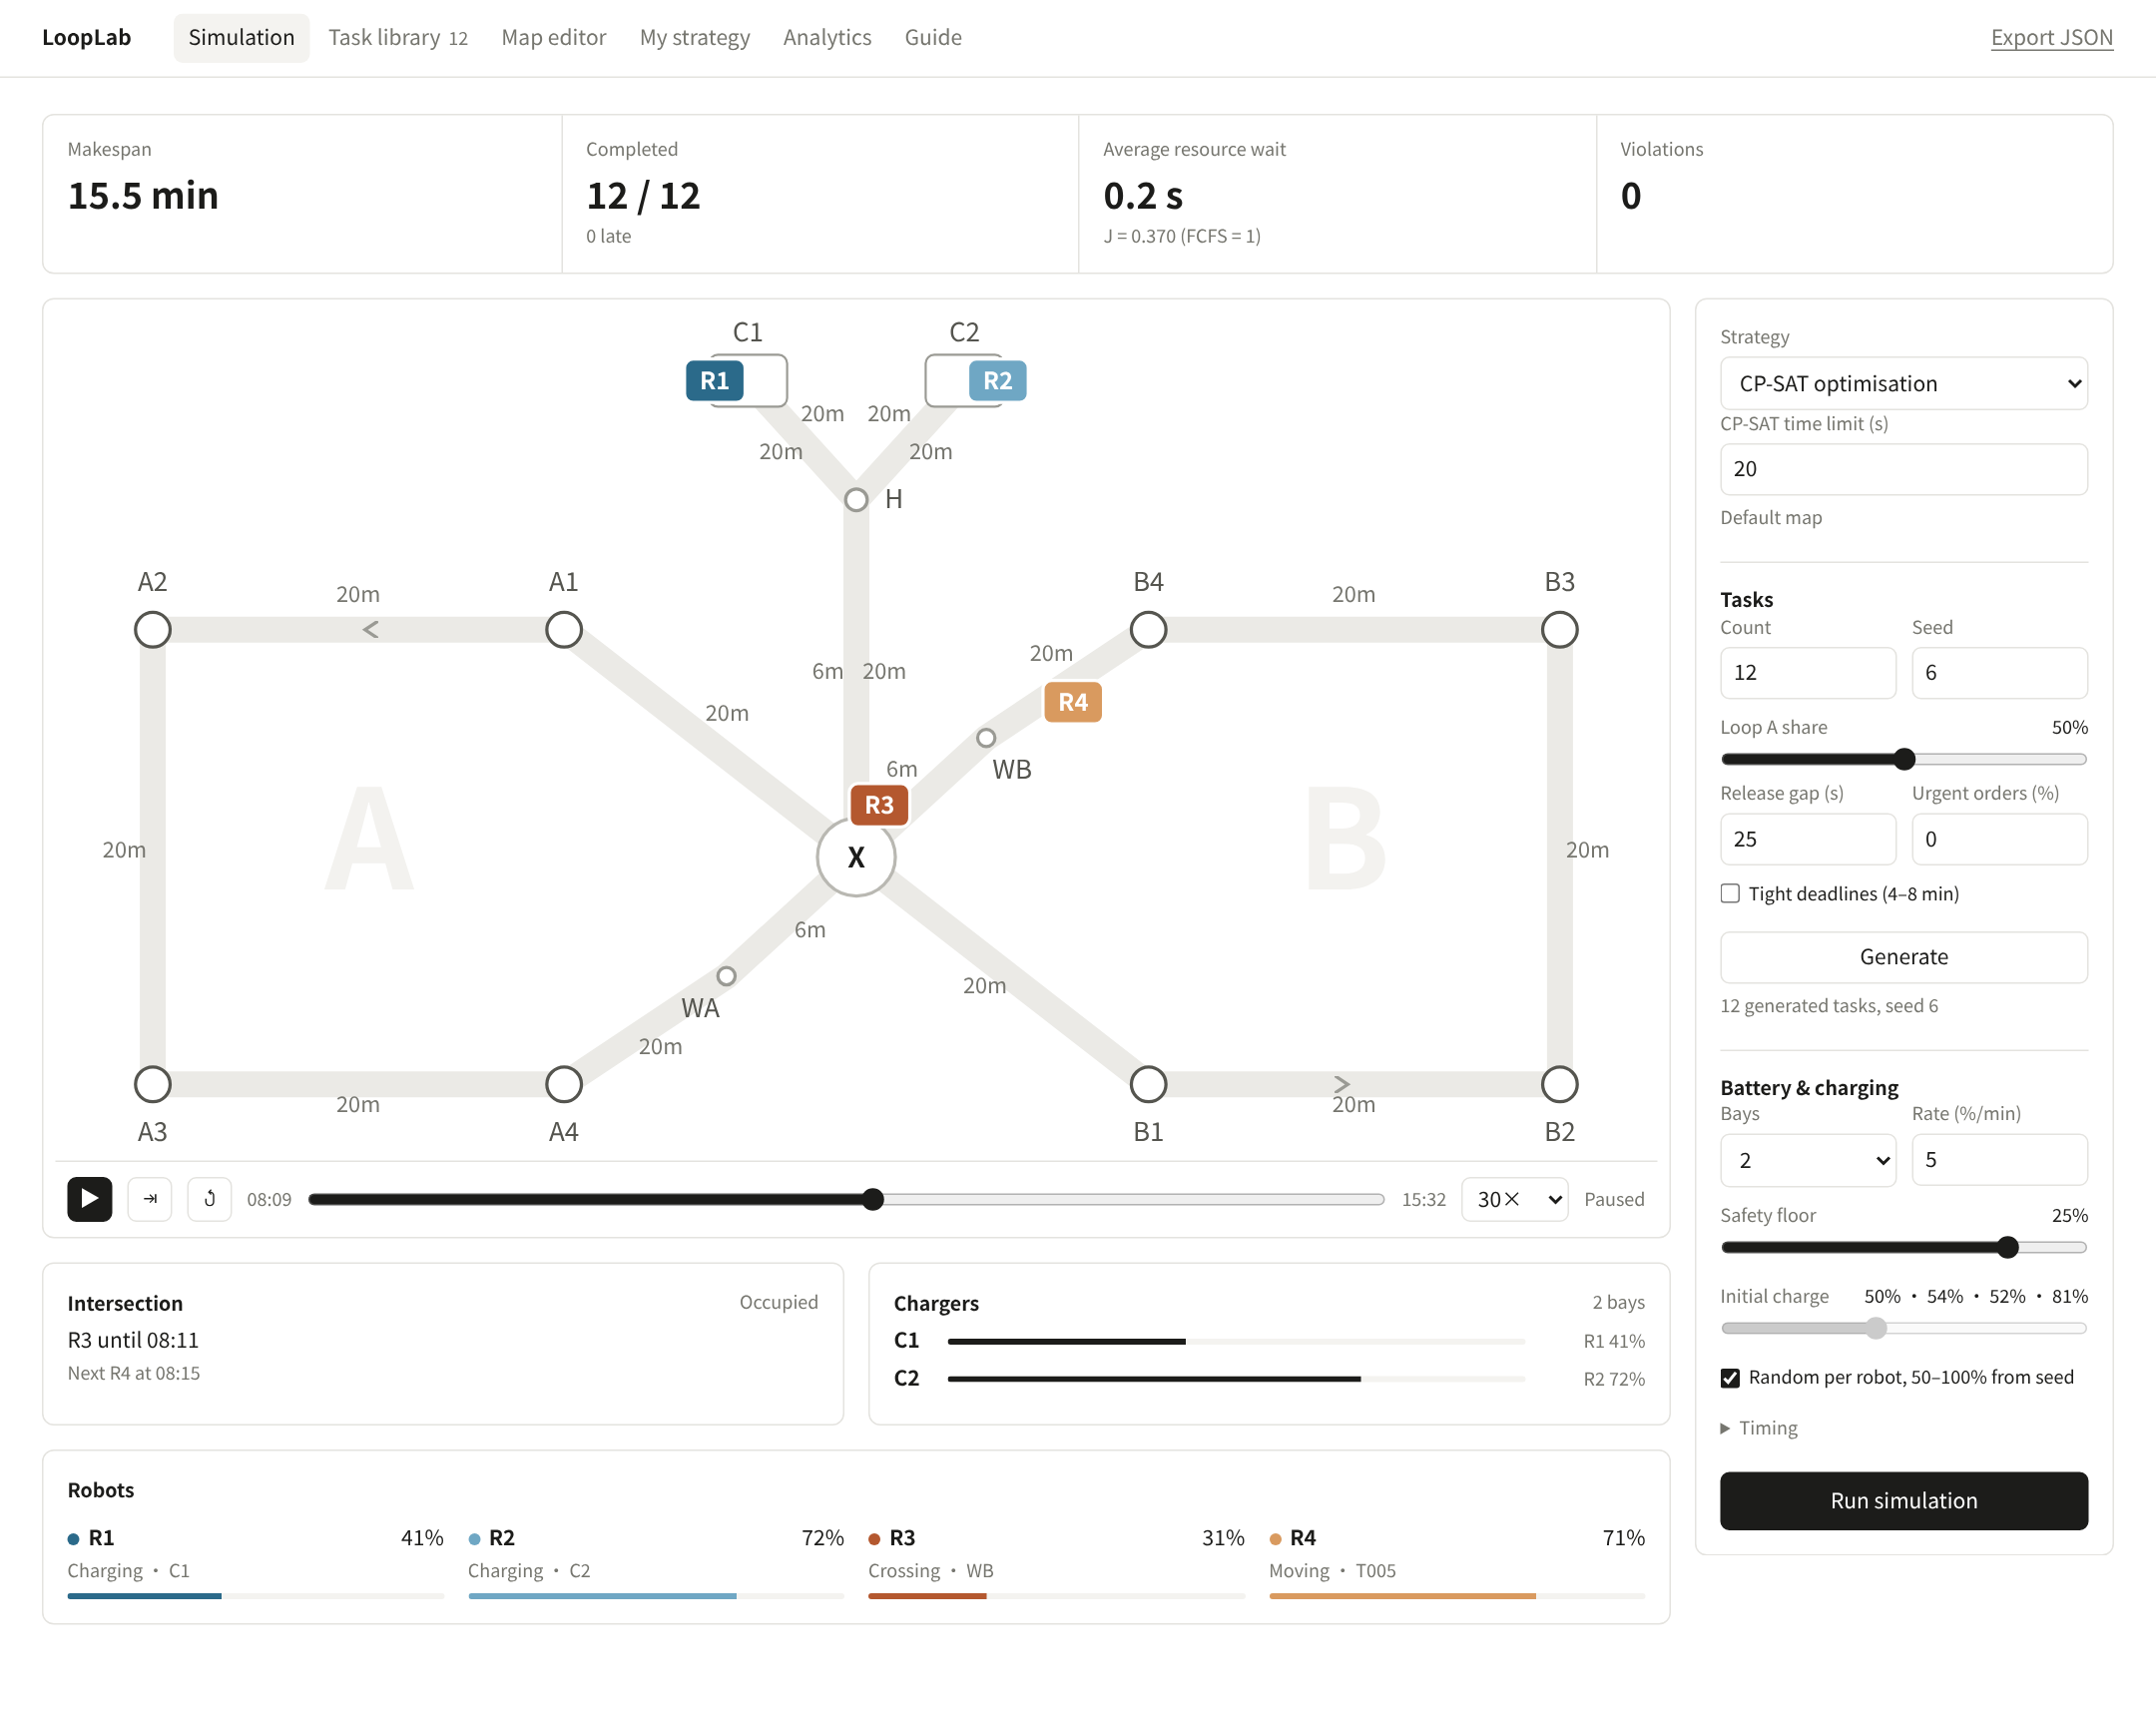
\includegraphics[width=0.9\linewidth]{ui_replay.png}
\caption{二维网页应用正在回放调度算例（第~\ref{sec:case}~节）的 CP-SAT 调度，暂停在 08:09（489\,s）。R3 位于 X 内
（交叉口面板显示其占用到 08:11，下一个是 R4），R1 和 R2 分别占用充电位 C1 和 C2，R4 正驶向 X 去执行任务 T005。
顶部显示本次运行的指标，包括相对 FCFS 的 $J = 0.370$。}
\label{fig:ui}
\end{figure}

\section{调度策略}

\subsection{基线策略}

\begin{enumerate}
\item \textbf{FCFS（先到先服务）}——按释放顺序处理任务；每个任务交给预计最早完成的兼容机器人；电量低于 20\pct\ 的机器人
  在下一个任务前先充电；交叉口时隙按预约顺序分配。
\item \textbf{分阶段}——方案中“先分配任务、再预约交叉口、最后安排充电”的分解。第一阶段按名义行驶时间做列表调度 \cite{pinedo2016} 来分配任务，
  忽略 X、充电位和电量；第二阶段按交叉口预约执行每台机器人的固定序列；第三阶段只在下一个任务否则会不安全时插入充电。
\item \textbf{截止时间优先 + 预约}——最早截止时间优先 \cite{liu1973,pinedo2016}（优先级打破平局），使用完整引擎的资源预约与电量检查。
\item \textbf{联合贪心}——对两台兼容机器人评估最多八个即将到来的任务，计入由此产生的交叉口和充电预约及充电插入，选出得分最低的候选：
  \[
    \text{score} = C_i + 3\,p_i T_i + 0.5\,W^{\text{new}} + 2\,E^{\text{new}},
  \]
  其中 $W^{\text{new}}$ 和 $E^{\text{new}}$ 为该候选新增的排队时间和能耗。
\end{enumerate}

所有自动策略在接受任务前都保留电量储备：机器人必须能完成该任务、到达 H，并扛过当前已预约的充电排队以及为其他三台机器人预留的保守余量。
所有启发式规则都固定充电到 95\pct。

\subsection{CP-SAT 联合优化}

模型由 CP-SAT（Google OR-Tools~9.15）\cite{perron2023cpsat,ortools} 求解。完整模型见 \code{docs/optimizer\_model.md}，本节给出概要。关键观察是：路线固定，因此一台机器人任意两个相邻作业之间的行驶时间、
能耗以及\emph{经过 X 的次数}都可预先算出。每台机器人 $k$ 对应一个图 $V_k = \{0\} \cup I_k \cup Q_k$，顶点包括表示当前状态的
起点 $0$、其环路上的所有任务 $I_k$，以及可选的充电访问 $Q_k$。

\paragraph{决策变量。}
$x_{ik} \in \{0,1\}$ 表示任务 $i$ 分配给机器人 $k$；弧变量 $a_{kab} \in \{0,1\}$ 选择每个顶点的后继；$s_i, c_i$ 为任务开始与完成时间；
对每次通过 $r$，$e_{kr}$ 为进入时间，$w_{kr} \ge 0$ 为在 X 前的等待，离开时间 $l_{kr} = e_{kr} + \tau_r$；对每次充电访问 $q$，
有是否存在变量 $y_{kq}$、充电位选择变量 $b_{kqp}$、在 H 的排队时间 $w^{C}_{kq}$、充电开始时间 $u_{kq}$ 与时长 $D_{kq}$；
每个顶点在到达后和服务后的电量；迟到时间 $T_i$ 与完工时间 $C_{\max}$。

\paragraph{约束。}
\begin{align}
&\textstyle\sum_{k} x_{ik} = 1 \quad \forall i,
  \qquad \textsc{Circuit}\big(\{a_{kab}\}\big) \quad \forall k
  && \text{（分配）}\\
&a_{kab} = 1 \;\Rightarrow\; s_{b} \ge c_{a}, \qquad s_i \ge r_i
  && \text{（先后与释放）}\\
&e_{kr} = \text{arrival}_{kr} + w_{kr}, \qquad l_{kr} = e_{kr} + \tau_r
  && \text{（通过时间）}\\
&\textsc{NoOverlap}\big(\{[e_{kr},\, l_{kr} + 2\beta)\}_{k,r}\big)
  && \text{（X 互斥）}\\
&u_{kq} = h_{kq} + w^{C}_{kq} + \tau_{Hp}, \qquad
  S^{-}_{kq} = S_{H,kq} - \rho_w w^{C}_{kq} - g_{Hp} \ge S_{\min}
  && \text{（H 处排队）}\\
&S^{+}_{kq} = S^{-}_{kq} + \rho_c D_{kq} \le 100, \qquad
  \textstyle\sum_p b_{kqp} = y_{kq}
  && \text{（充电量）}\\
&\textsc{NoOverlap}\big(\{[u_{kq},\, u_{kq} + D_{kq}) : b_{kqp} = 1\}\big) \quad \forall p
  && \text{（充电位互斥）}\\
&\mathit{soc}_{\text{out}} = \mathit{soc}_{\text{in}} - \textstyle\sum g_{ab} - \sum g_h
  - \rho_w \sum w \;\ge\; S_{\min}
  && \text{（能耗）}\\
&\mathit{soc}_{\text{last}(k)} \ge S_{\min} + G_{k \to H \to p} + \rho_w\, \bar W_{\text{queue}} + \delta
  && \text{（末端储备）}
\end{align}
其中 $\tau$ 和 $g$ 为边的时长与能耗，$g_h$ 为装卸能耗，$h_{kq}$ 和 $S_{H,kq}$ 为到达 H 的时间与电量，$G_{k\to H\to p}$ 为从机器人最后
一个站点到最近充电位的能耗，$\bar W_{\text{queue}} = 3\,(95 - S_{\min})/\rho_c$ 为启发式规则预留的“排在另外三次完整充电之后”的等待时间，
$\delta = 0.5\pct$ 为小余量。每条弧上和每个任务内部的每次通过都是一个可选区间 \cite{laborie2018}，只有选中对应弧时才存在；等待发生在进入前的等待点
（$W_A$、$W_B$ 或 H），绝不在 X 内。机器人充电结束后立即离开充电位，充电量 $\rho_c D_{kq}$ 是决策变量，而启发式规则固定充到 95\pct。
末端储备与启发式规则在接受任何任务前所检查的条件相同。若没有余量 $\delta$，最优解会恰好落在边界上，随后被仿真器的检查拒绝，
因为该检查在前往 H 的途中还会计入在 X 前排队的耗电。迟到时间与完工时间通过 $T_i = \max(0, c_i - d_i)$ 和
$C_{\max} = \max_i c_i$ 线性化（\code{AddMaxEquality}）。

目标函数正是式~\eqref{eq:J} 中的归一化 $J$；其参考值 $\hat R_k$ 在求解前算出，是常数，因此 $J$ 保持线性。时间以毫秒为单位、
电量以整数单位表示，所有时长和能耗都\emph{向上}取整，保证整数可行的调度在精确仿真器中仍然可行。模型以联合贪心的调度作为初始解
（\code{AddHint}）。

\paragraph{解码。}求解器的决策（序列、通过进入时间、充电位、充电开始时间与目标电量）通过仿真器自己的规划器重放，因此返回调度中的
时间和能耗都来自仿真器，且结果必须通过独立验证器。若解码后的调度比初始解差或未通过验证，则返回初始解并记录回退，
因此 CP-SAT 报告的调度绝不会比联合贪心差。

\paragraph{搜索。}CP-SAT 使用 8 个并行工作线程。只用一个线程时，求解器在 40 个任务的实例上运行约两分钟也没有改进初始解；
而并行组合（主要由大邻域搜索 \cite{shaw1998} 线程完成改进）在相同时间内显著改进了它。在小实例（4--6 个任务）上模型可证明最优，并与解析下界一致
（单元测试）。在实际规模上下界仍然较弱，因此结果是优质的可行解，而非已证明的最优解。

\subsection{滚动时域再优化}

离线优化假设所有任务在时刻 0 已知。滚动策略去掉了这一假设：任务只在其释放时刻才可见，计划在后退的时域上反复重算 \cite{sethi1991,mayne2000}（算法~\ref{alg:rolling}）。

\begin{algorithm}[H]
\caption{滚动时域 CP-SAT}
\label{alg:rolling}
\begin{algorithmic}[1]
\State $t \gets 0$
\While{仍有未完成任务}
  \State $\mathcal{K} \gets$ 截至 $t$ 已释放且尚未开始的任务
  \State $\mathcal{W} \gets$ $\mathcal{K}$ 中按紧急程度排序的任务，直到每条环路约 600\,s 的工作量
  \State $\hat R \gets$ 从当前状态继续、仅针对 $\mathcal{K}$ 的 FCFS 参考值 \Comment{在线归一化}
  \State plan $\gets$ 从机器人当前状态出发、对 $\mathcal{W}$ 求解 CP-SAT，已承诺的 X 与充电位预约固定
         （1 个线程，确定性预算约 0.5\,s，初始解为联合贪心）
  \State 承诺 plan 中所有在 $t + 60$\,s 之前开始的作业，并冻结其预约
  \State $t \gets t + 60$\,s
\EndWhile
\end{algorithmic}
\end{algorithm}

已承诺的动作不再修改。每个窗口求解都要求每台机器人最后计划的作业之后保留末端储备，使下一个窗口不会陷入电量死局。
归一化本身也是在线的：参考值只来自截至当前已知任务的 FCFS 调度。早期版本使用了全实例参考值，代码审查发现这会改变决策，
即泄露了未来信息。最终调度与其他策略一样，用全实例的 $J$ 评分。

\section{调度算例}
\label{sec:case}

本节完整跟踪一个小实例，使汇总数字背后的具体决策清晰可见。该实例有 12 个任务（随机种子 6，释放间隔取 25\,s 而非默认的 12\,s，因此均在前 280\,s 内释放；区域 A 五个、
区域 B 七个），R1--R4 的初始电量为 50.1、53.9、52.2 和 80.8\pct（即应用中该种子的“每台机器人随机”初始电量），安全阈值 25\pct，
两个充电位，其余参数取默认值。我们比较 FCFS 与 CP-SAT；CP-SAT 使用单线程和确定性时间预算，因此调度可以复现。两份调度都通过了
独立验证器，下文所有数字都可由 \code{report/case\_study.py} 重新生成。

\paragraph{任务分配。}表~\ref{tab:case-orders} 列出了每个任务及服务它的机器人。任务只能分给其所在区域的两台机器人之一，但两种方法的
分法不同。FCFS 把 T012（截止于 547\,s）分给 R2，而 R2 必须先充电，因此 T012 要等 R2 充电 11 分钟之后才完成，迟到 430\,s。
CP-SAT 同样先派 R2 去充电，但让 R1 先完成 T012（201\,s 完成）再去充电。在区域 B，R4 服务四个任务，其中两个是在 R3 充电期间完成的。

\begin{table}[H]
\centering\small
\setlength{\tabcolsep}{4.5pt}
\begin{tabular}{llrrr rrr rrr}
\toprule
& & & & & \multicolumn{3}{c}{FCFS} & \multicolumn{3}{c}{CP-SAT} \\
\cmidrule(lr){6-8}\cmidrule(lr){9-11}
任务 & 环路：路线 & $r_i$ & $d_i$ & $p_i$ & 机器人 & $C_i$ & $T_i$ & 机器人 & $C_i$ & $T_i$ \\
\midrule
\inputrows{../results/case/tasks.tex}
\bottomrule
\end{tabular}
\caption{调度算例的任务及其分配（$r_i$ 释放时间，$d_i$ 截止时间，$p_i$ 优先级，$C_i$ 完成时间，$T_i$ 迟到时间；单位为秒）。}
\label{tab:case-orders}
\end{table}

\paragraph{交叉口。}表~\ref{tab:case-robots} 给出 CP-SAT 调度中每次进入 X 的时刻。每次通过占用 X 6\,s，下一次通过最早只能在其结束
4\,s（$2\beta$）之后开始。调度中最紧凑的一对恰好达到这一下限：R3 在去充电途中于 491.6\,s 离开 X，R4 于 495.6\,s 进入。两份调度中唯一
一次交叉口等待发生在 FCFS 中：R2 在 80\,s 通过，同时到达 $W_A$ 的 R1 等待 10\,s（6\,s 通过时间加 4\,s 间隔）。CP-SAT 让 R1 在 140\,s
才通过 X，从而避免了这次等待。

\begin{table}[H]
\centering\small
\begin{tabular}{llcp{5.5cm}rrr}
\toprule
机器人 & 环路 & 任务数 & 进入 X 的时刻（s） & 初始电量 & 最低电量 & 最终电量 \\
\midrule
\inputrows{../results/case/robots.tex}
\bottomrule
\end{tabular}
\caption{CP-SAT 调度的逐台机器人情况：进入 X 的时刻（上标 c：前往充电区途中；H：从充电区返回；其余为沿环路行驶）以及电量（\%）。}
\label{tab:case-robots}
\end{table}

\paragraph{充电。}两种方法都充电三次（表~\ref{tab:case-charging}），但方式截然不同。FCFS 总是充到 95\pct。R2 从 126\,s 到 770\,s
占用 C1。R1 在 116\,s 到达 H，但 C2 已被 R3 从 281\,s 起预约，而从 37\pct\ 充满约需 12 分钟，两个充电位都放不下，于是 R1 在 H 等待
634\,s，并在 770\,s R2 离开时进入 C1。CP-SAT 则只把每台机器人充到其剩余任务和末端储备所需的电量：R2 充到 75.3\pct，R1 充到 62.7\pct，
R3 充到 52.1\pct。总充电时间从 2049\,s 降到 1151\,s，充电位之间也没有空档：R3 在 512\,s 到达 H，等待 2.4\,s 后于 534\,s 进入 C2，
恰好是 R2 离开的时刻。

\begin{table}[H]
\centering\small
\begin{tabular}{lllrrcrc}
\toprule
方法 & 机器人 & 充电位 & 到达 H（s） & 排队（s） & 充电区间（s） & 时长（s） & 电量（\%） \\
\midrule
\inputrows{../results/case/charging.tex}
\bottomrule
\end{tabular}
\caption{调度算例的充电操作：到达充电区入口 H 的时刻、在 H 的排队时间、在充电位内的时间段以及充电前后的电量。}
\label{tab:case-charging}
\end{table}

\paragraph{电量变化。}图~\ref{fig:case} 以甘特图展示两份调度，下方为电量曲线。在 FCFS 下，电量以很长的直线段充到 95\pct，R1 在 H
等待时电量缓慢下降。CP-SAT 更充分地利用了可用电量：R1 在到达 C1 时达到最低值 25.9\pct，仅比阈值高 0.9 个百分点。所有机器人最终电量都在
42 到 52\pct\ 之间，不低于末端储备（安全阈值、到达充电位所需的能耗以及排队余量）。两份调度中都没有机器人低于安全阈值。

\begin{figure}[H]
\centering
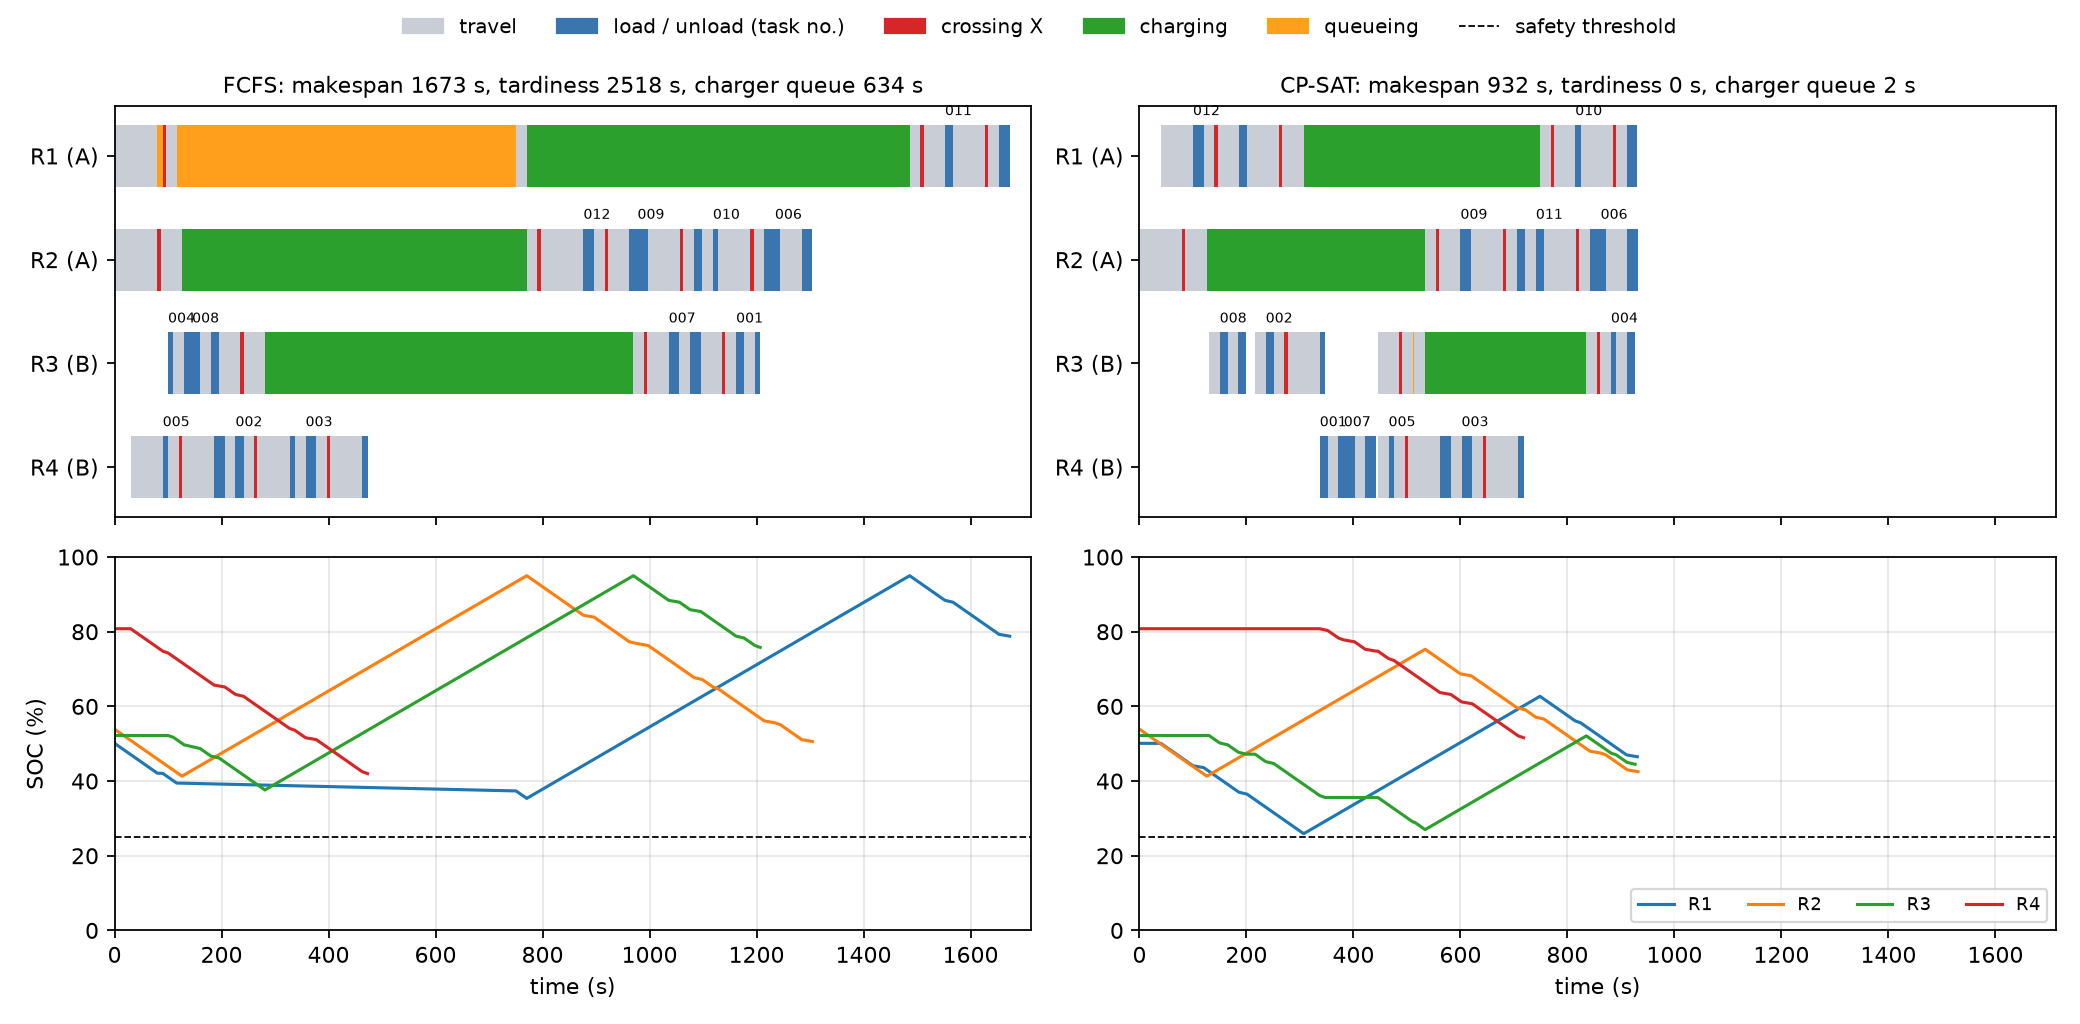
\includegraphics[width=\linewidth]{case_study.png}
\caption{调度算例。上：每台机器人的甘特图（灰色为行驶，蓝色为装/卸货并标注任务编号，红色为通过 X，绿色为充电，橙色为排队）。
下：各机器人电量及 25\pct\ 安全阈值。左为 FCFS，右为 CP-SAT。}
\label{fig:case}
\end{figure}

\paragraph{结果。}表~\ref{tab:case-summary} 汇总了结果。CP-SAT 按时完成全部任务，比 FCFS 早 12 分钟结束，能耗少 8\pct，几乎没有排队。
图~\ref{fig:case-ui} 是同一份 CP-SAT 调度在网页应用分析页中的显示，其中的甘特图、电量曲线、X/C1/C2 预约时间轴和配送表都与上面的表格一致。

\begin{table}[H]
\centering\small
\begin{tabular}{lrr}
\toprule
指标 & FCFS & CP-SAT \\
\midrule
完工时间 $C_{\max}$（s） & 1673 & 932 \\
总迟到时间 $\sum_i T_i$（s） & 2518 & 0 \\
迟到任务数 & 7 & 0 \\
在 X 前 / 在 H 的排队（s） & 10 / 634 & 0 / 2.4 \\
能耗（\%） & 160.5 & 147.8 \\
充电次数 & 3 & 3 \\
最低电量（\%） & 35.4 & 25.9 \\
$J$（式~\ref{eq:J}） & 1.000 & 0.370 \\
\bottomrule
\end{tabular}
\caption{调度算例汇总。}
\label{tab:case-summary}
\end{table}

\begin{figure}[!htbp]
\centering
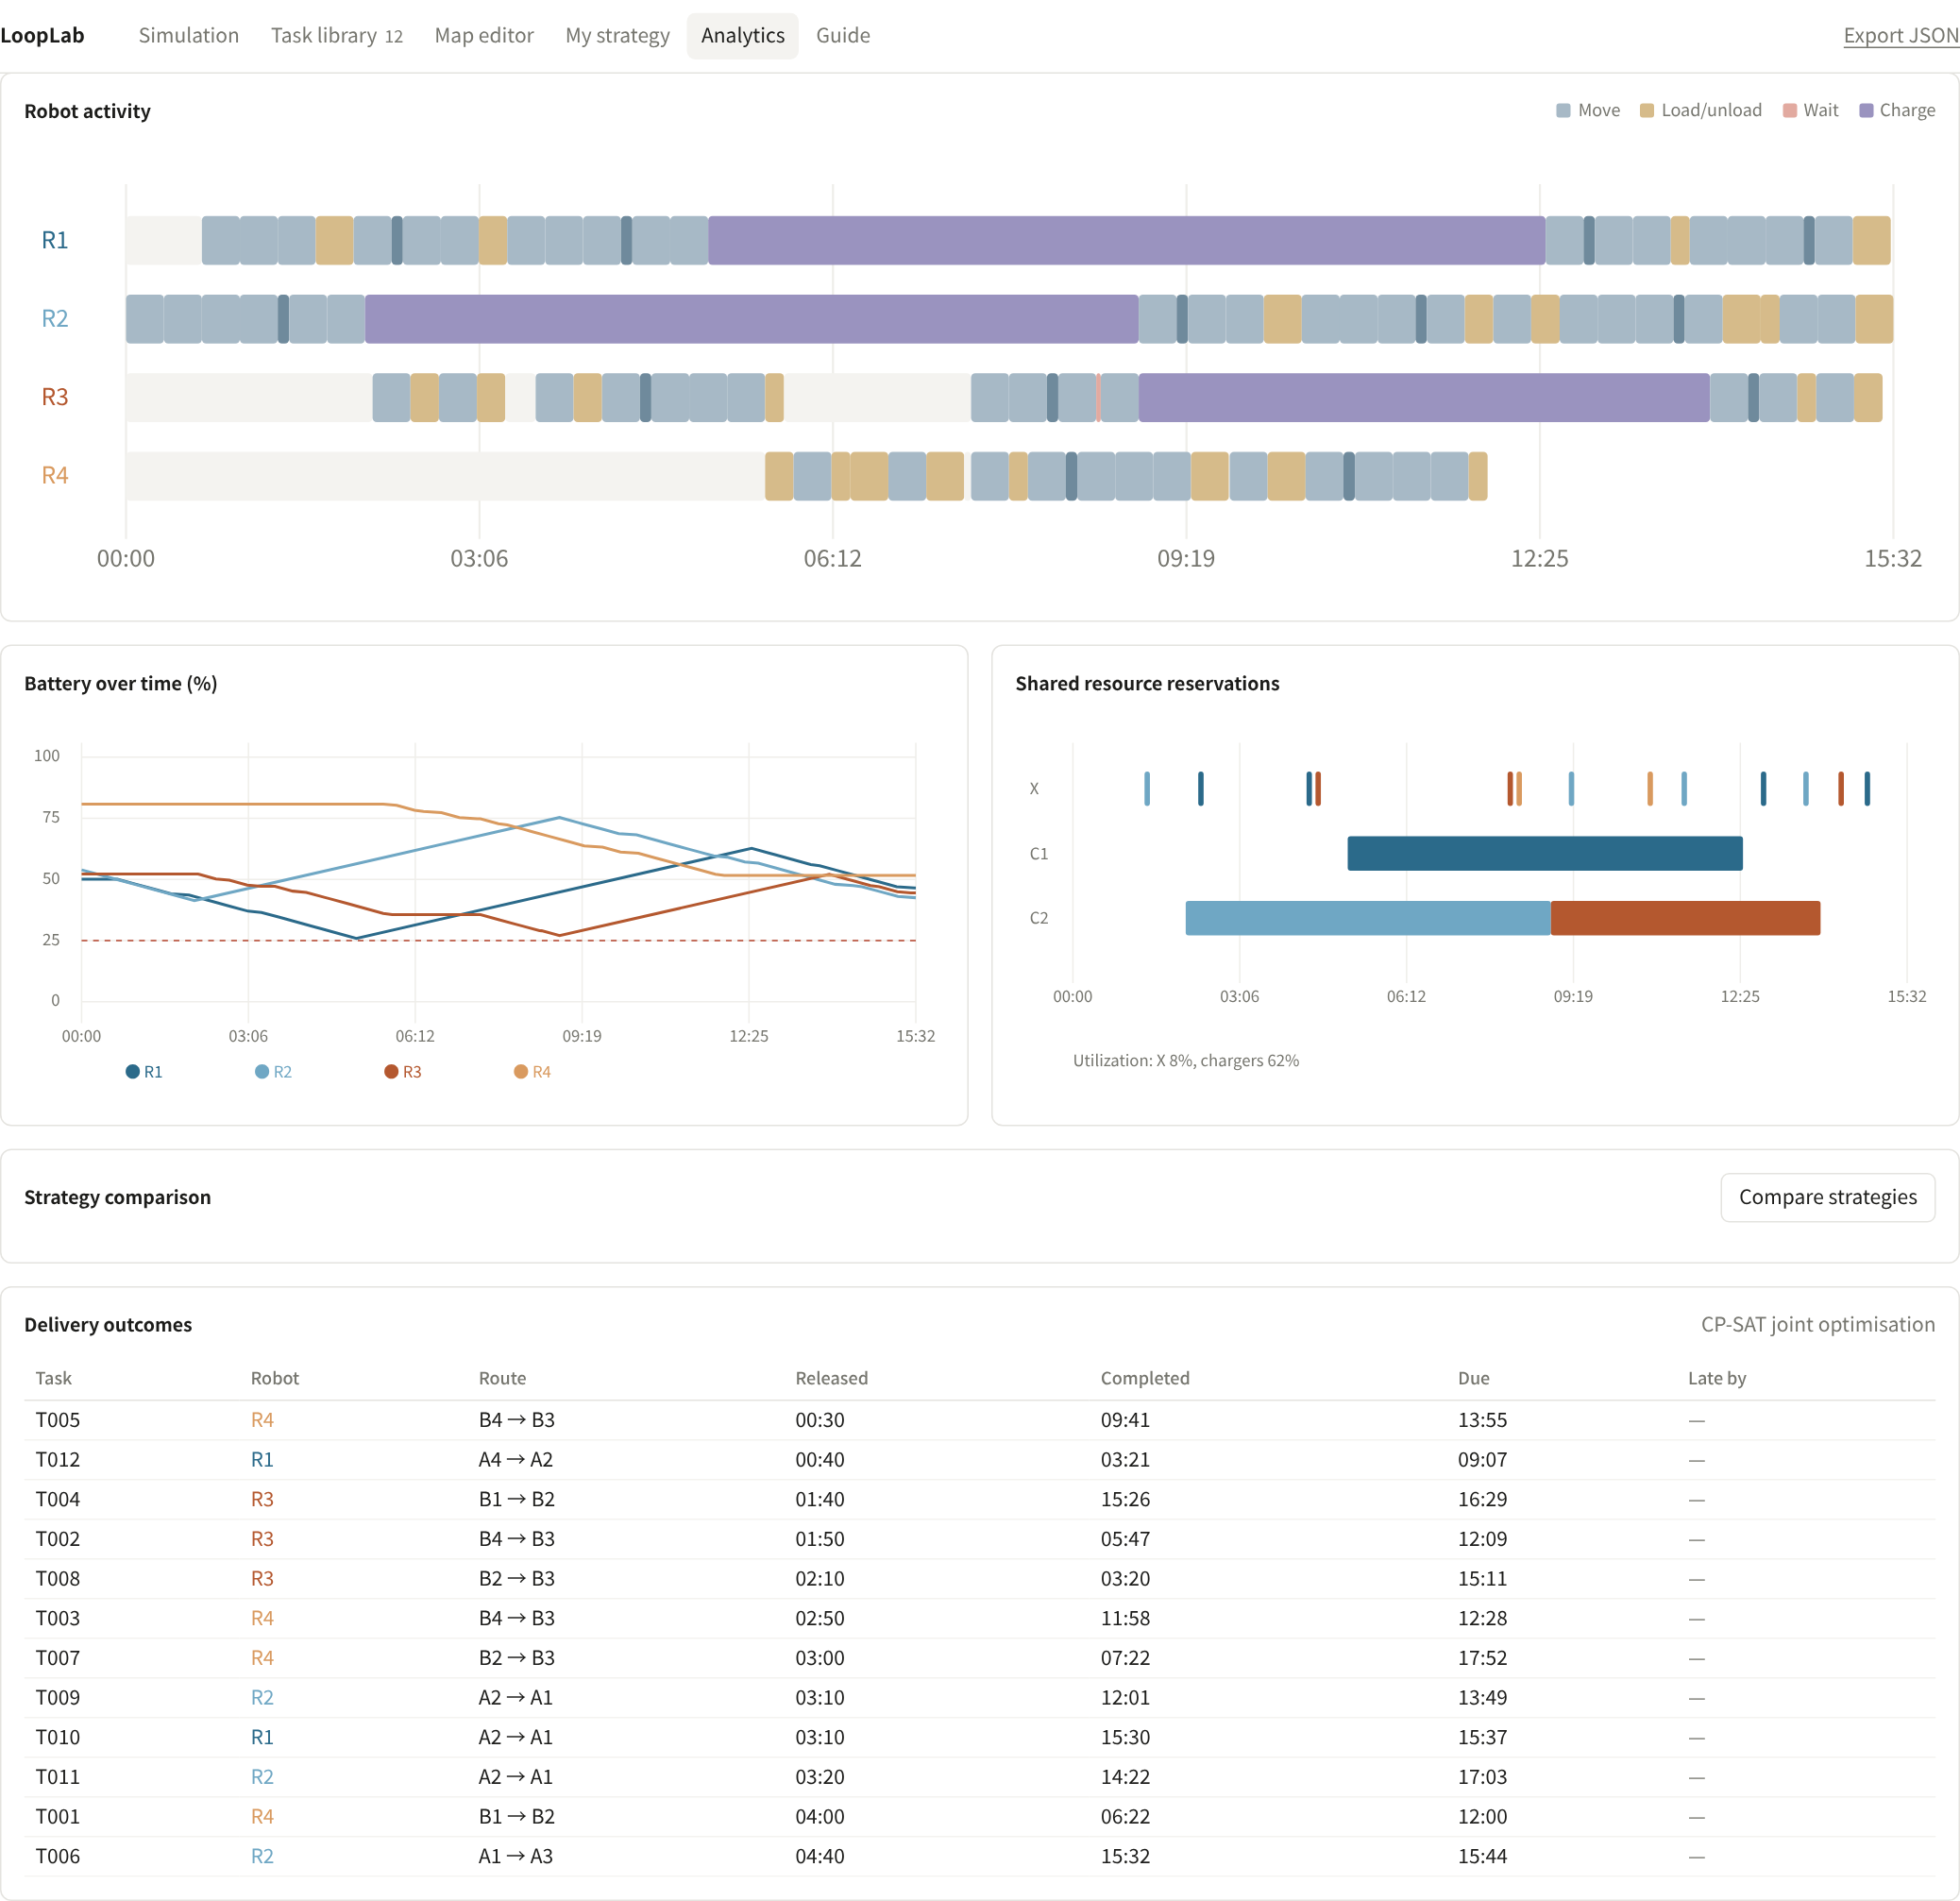
\includegraphics[width=0.88\linewidth]{ui_analytics.png}
\caption{调度算例中 CP-SAT 调度在网页应用分析页中的显示：机器人活动、电量随时间变化、X/C1/C2 预约以及配送结果。}
\label{fig:case-ui}
\end{figure}

\section{实验}

\subsection{实验设置}

方案中的实验计划由 \code{experiments.py} 执行。每种配置使用种子 1--10；对同一种子，全部七种策略（六种策略加上第~\ref{sec:reserve}~节的
消融实验）得到完全相同的任务列表、配置和固定种子的初始电量。基础设置为 40 个任务、2 个充电位、10\pct\ 安全阈值、区域任务比例 1:1、
无紧急任务；每个实验只改变一个因素（表~\ref{tab:exp}）。

\begin{table}[H]
\centering\small
\begin{tabular}{ll}
\toprule
实验 & 设置 \\
\midrule
算法比较 & 基础设置 \\
任务负载 & 20、40、60 个任务 \\
充电资源 & 1 或 2 个充电位 \\
区域不平衡 & A:B = 1:1、2:1、3:1 \\
安全阈值 & 10、20、30\pct \\
动态任务 & 增加 0、10、20\pct\ 紧急任务（释放后 3--6\,min 截止，优先级 4--5） \\
\bottomrule
\end{tabular}
\caption{实验计划。}
\label{tab:exp}
\end{table}

在多个实验中重复出现的相同实例（即基础设置）只求解一次，共计 10 种不同设置 $\times$ 10 个种子 $\times$ 7 种策略 $=$ 700 次运行。
每次运行记录 $J$ 及其四个原始项、迟到任务比例、X 与充电位的排队时间、能耗、充电次数和运行时间。由于不同种子的难度差别很大，
表中还给出同一实例上 $J$ 相对 FCFS 的\emph{配对}变化。

\emph{计算环境。}四种启发式规则和滚动策略都是确定性的（滚动求解受 CP-SAT 确定性时间约束，而非墙钟时间），因此其调度与机器无关；
这一点已通过在两台不同机器上逐位复现一次滚动运行得到验证。CP-SAT 受墙钟时间约束（120\,s，8 个线程），因此依赖硬件；所有 CP-SAT
运行都使用同一机型（Google Colab 高内存 CPU 虚拟机，8 vCPU Intel Xeon @ 2.20\,GHz，OR-Tools 9.15），每台虚拟机同一时间只运行一个求解。

\emph{公平性说明。}启发式规则和离线 CP-SAT 预先知道全部任务列表（但不会在释放前开始任何任务）；滚动策略是唯一真正在线的方法。
所有策略在时域末端保留相同的电量储备（每台执行任务的机器人都必须能排在满队列之后到达充电位；没有任务的机器人在任何策略下都不移动）。
第一次运行的离线 CP-SAT 没有该储备，作为消融实验 \code{cpsat-nores} 保留；它常常以接近安全阈值的电量结束，并经常完全不充电，
从而夸大了优势，第~\ref{sec:reserve}~节对此做了量化。启发式规则总是充到 95\pct，而 CP-SAT 自行选择充电量。

\subsection{算法比较（基础设置）}

\begin{table}[H]
\centering\small
\setlength{\tabcolsep}{3.5pt}
\resizebox{\linewidth}{!}{%
\begin{tabular}{lrrrrrrrr}
\toprule
策略 & $J$ & 相对 FCFS & 迟到 & 迟到时间 & 完工时间 & 充电 & 能耗 & 运行时间\textsuperscript{a} \\
 & & 均值 / 中位数 & 比例 & (s) & (s) & 次数 & (\%) & \\
\midrule
FCFS & 1.000 & -- & 52\pct & 26\,028 & 3\,233 & 5.0 & 443 & $<0.1$\,s \\
分阶段 & 1.067 & $+7$ / $+2$\pct & 51\pct & 27\,264 & 3\,441 & 5.4 & 449 & $<0.1$\,s \\
截止时间优先 + 预约 & 1.003 & $0$ / $-4$\pct & 51\pct & 25\,994 & 3\,210 & 4.9 & 438 & $<0.1$\,s \\
联合贪心 & 0.793 & $-21$ / $-23$\pct & 37\pct & 17\,826 & 3\,021 & 3.9 & 386 & 0.3\,s \\
滚动 CP-SAT（在线） & 0.636 & $-36$ / $-37$\pct & 37\pct & 15\,651 & 2\,741 & 4.3 & 389 & 49\,s \\
\textbf{CP-SAT} & \textbf{0.468} & $\mathbf{-53}$ / $\mathbf{-54}$\pct & 33\pct & 9\,934 & 2\,317 & 4.2 & 359 & 121\,s \\
CP-SAT 无储备（消融） & 0.349 & $-65$ / $-64$\pct & 23\pct & 5\,032 & 1\,732 & 2.0 & 316 & 121\,s \\
\bottomrule
\end{tabular}}
\caption{基础设置（40 个任务、2 个充电位、10\pct\ 阈值、1:1 区域）；10 个种子的均值，$J$ 相对 FCFS 的配对变化以“均值 / 中位数”给出。
\textsuperscript{a}每个实例实测的墙钟时间（CP-SAT 预算为 120\,s；滚动策略在 2 vCPU 虚拟机上运行）。完整表格见 \code{results/results.md}。}
\label{tab:base}
\end{table}

\begin{figure}[H]
\centering
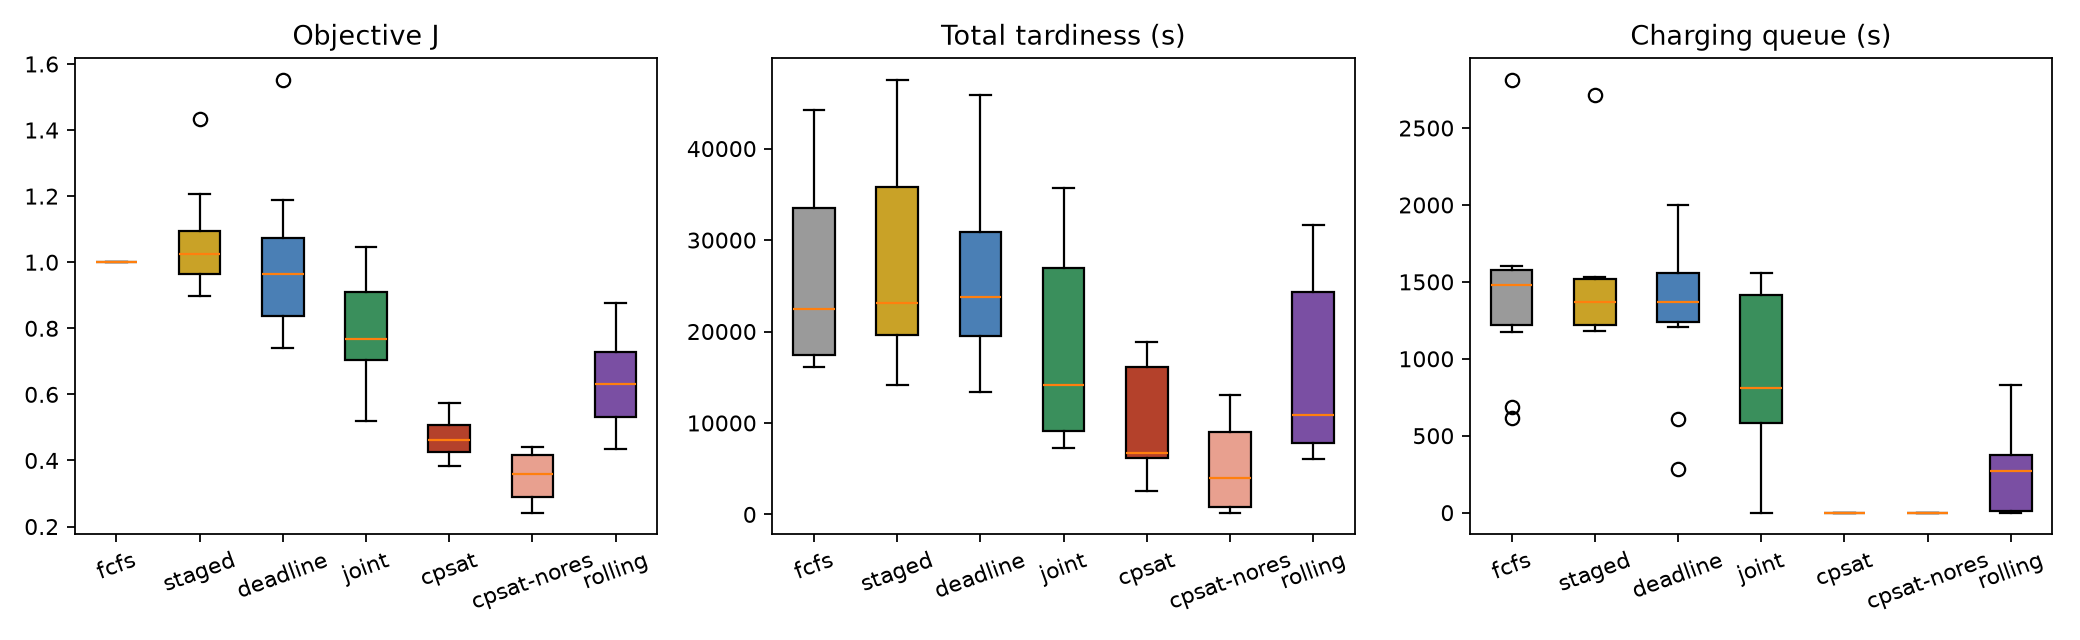
\includegraphics[width=\linewidth]{algorithms.png}
\caption{基础设置，10 个种子：各策略的目标值 $J$、总迟到时间和充电排队时间。}
\label{fig:algorithms}
\end{figure}

全部 700 次运行都得到了通过验证、电量安全的调度；没有任何策略在任何实例上失败。均值和中位数给出相同的性能层级，并在大多数单个种子上成立
（图~\ref{fig:algorithms}）：三种单一规则基线彼此相差不超过 $\pm 7$\pct（其内部顺序有所不同：按均值 FCFS 略优于截止时间优先，按中位数
截止时间优先领先 4\pct），联合贪心约好五分之一，滚动策略约好三分之一，离线 CP-SAT 约好一半。离线 CP-SAT 从未回退到初始解，但最优性间隙
仍然较大（基础设置：中位数 58\pct，范围 51--70\pct；全部 100 个实例：中位数 63\pct，范围 18--76\pct）：回路模型的下界较弱，
因此这些是优质可行解，而非已证明的最优解。

\subsection{敏感性实验}

表~\ref{tab:sens} 给出 $J$ 相对 FCFS 的配对变化中位数。均值见 \code{results/results.md}；在 FCFS 某项接近零而放大个别运行的情况下
（第~\ref{sec:norm}~节），均值与中位数差别很大，例如 20 个任务时分阶段和截止时间优先的均值分别为 $+81$\pct\ 和 $+134$\pct，
而中位数为 $+7$\pct\ 和 $+10$\pct。

\begin{table}[H]
\centering\small
\begin{tabular}{llrrrrr}
\toprule
实验 & 设置 & 分阶段 & 截止时间优先 & 联合贪心 & 滚动 & CP-SAT \\
\midrule
\multirow{3}{*}{任务负载} & 20 个任务 & $+7$ & $+10$ & $-30$ & $-43$ & $-62$ \\
 & 40 个任务 & $+2$ & $-4$ & $-23$ & $-37$ & $-54$ \\
 & 60 个任务 & $+8$ & $+10$ & $-16$ & $-18$ & $-47$ \\
\midrule
\multirow{2}{*}{充电位} & 1 个 & $+45$ & $-1$ & $-20$ & $-28$ & $-60$ \\
 & 2 个 & $+2$ & $-4$ & $-23$ & $-37$ & $-54$ \\
\midrule
\multirow{2}{*}{区域不平衡 A:B} & 2:1 & $+4$ & $+2$ & $-15$\textsuperscript{b} & $-25$ & $-48$ \\
 & 3:1 & $0$ & $-6$ & $-29$ & $-30$ & $-47$ \\
\midrule
\multirow{2}{*}{安全阈值} & 20\pct & $+2$ & $+11$ & $-18$ & $-16$ & $-51$ \\
 & 30\pct & $+17$ & $-1$ & $-13$ & $-16$ & $-52$ \\
\midrule
\multirow{2}{*}{紧急任务} & +10\pct & $+1$ & $-3$ & $-12$ & $-24$ & $-52$ \\
 & +20\pct & $+4$ & $-5$ & $-8$ & $-20$ & $-50$ \\
\bottomrule
\end{tabular}
\caption{$J$ 相对 FCFS 的配对变化中位数（\%），每格 10 个种子。\textsuperscript{b}均值为 $+19$\pct：有一个种子的 $J = 3.7$，
尽管联合贪心在该实例上的完工时间、迟到和能耗都优于 FCFS（第~\ref{sec:norm}~节）。}
\label{tab:sens}
\end{table}

\begin{figure}[H]
\centering
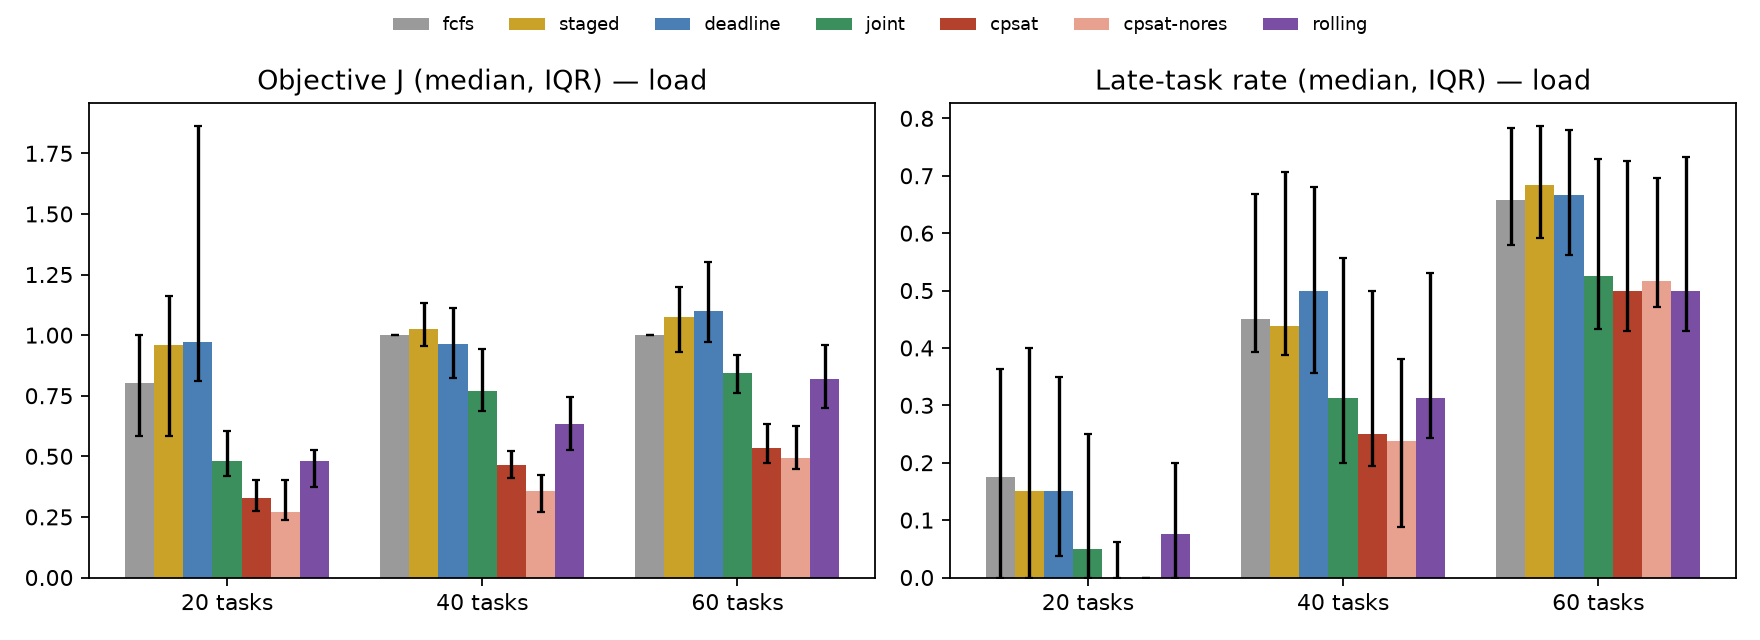
\includegraphics[width=\linewidth]{load.png}
\caption{任务负载实验：$J$ 与迟到任务比例的中位数及四分位距。}
\label{fig:load}
\end{figure}

\begin{itemize}
\item \textbf{任务负载。}随着任务增加，所有方法都变差，但启发式规则和滚动策略相对 FCFS 的优势缩小（$-43$\pct\ $\to$ $-18$\pct），
  而 CP-SAT 保持在 $-47$\pct\ 到 $-62$\pct（图~\ref{fig:load}）。60 个任务时每种方法都有一半以上的任务迟到（迟到比例 54--69\pct）；
  队伍已超出能力，充电（7--10 次，每次最长 17\,min）成为瓶颈资源。
\item \textbf{单个充电位。}FCFS 的充电排队从 1\,437\,s 增加到 4\,001\,s，分阶段基线大幅恶化（$+45$\pct）：它最后才决定充电，
  机器人会同时到达唯一的充电位。联合贪心和 CP-SAT 把充电与任务一起决定，保持了优势；CP-SAT 改进最多（$-60$\pct）。
\item \textbf{区域不平衡。}环路 A 的任务越多，所有方法的完工时间越长，因为 R1/R2 成为瓶颈。性能层级不变（CP-SAT 最好，其次是
  滚动和联合贪心，最后是单一规则基线），只是在基线层级内部，2:1 时截止时间优先按中位数略落后于 FCFS（$+2$\pct）。
\item \textbf{安全阈值。}阈值越高，所有方法都需要更多充电。CP-SAT 几乎不受影响（$-51$\pct\ / $-52$\pct），而滚动策略退回到联合贪心的水平
  （$-16$\pct）：它的每个窗口都必须以完整储备结束，在 20--30\pct\ 阈值下这会迫使其提前充电，而离线视角本可避免。
\item \textbf{紧急任务。}截止期短、优先级高的任务会使所有方法变差；离线 CP-SAT 保持约 $-50$\pct，滚动策略为 $-20$\pct\ 到 $-24$\pct。
  对紧急任务最直观的截止时间优先规则只改进 3--5\pct。
\end{itemize}

\begin{figure}[H]
\centering
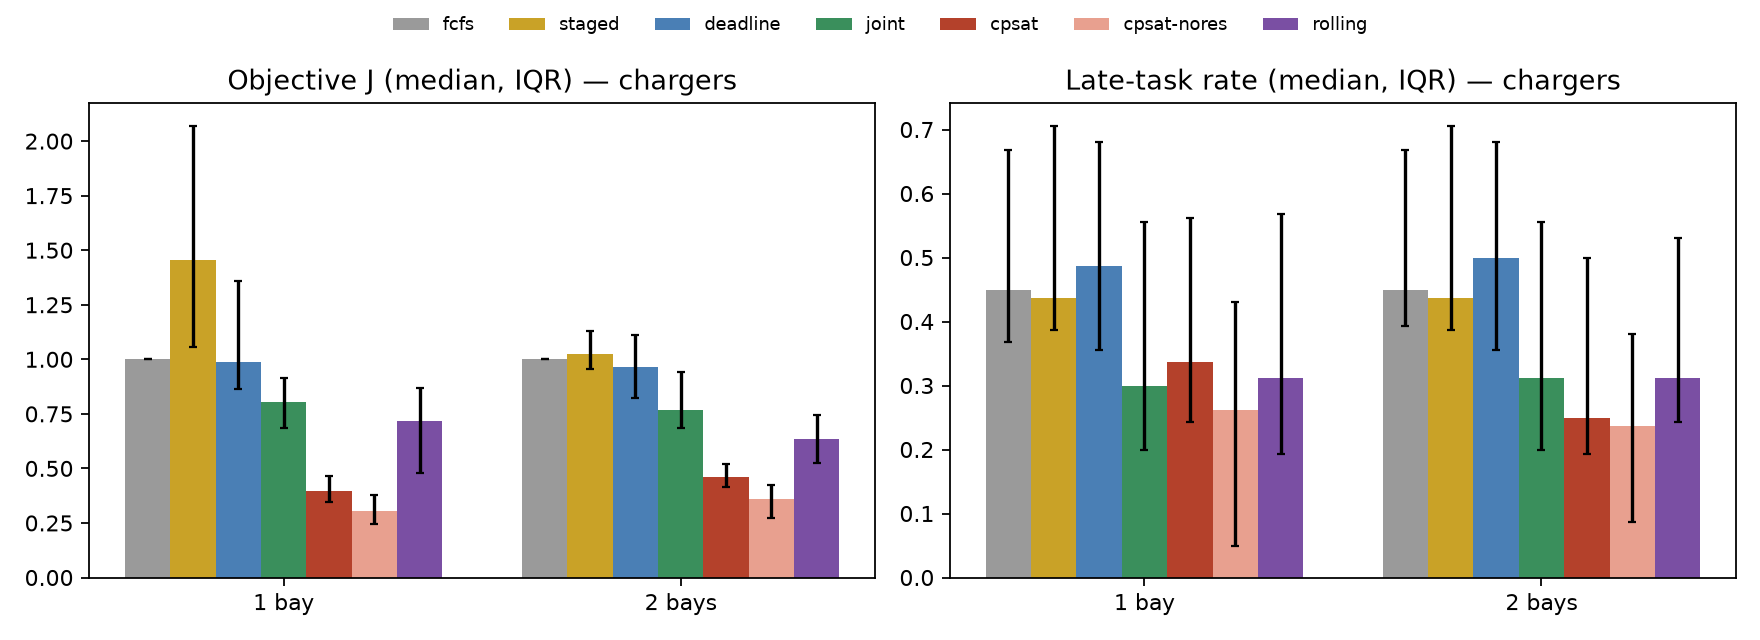
\includegraphics[width=0.92\linewidth]{chargers.png}\\[2pt]
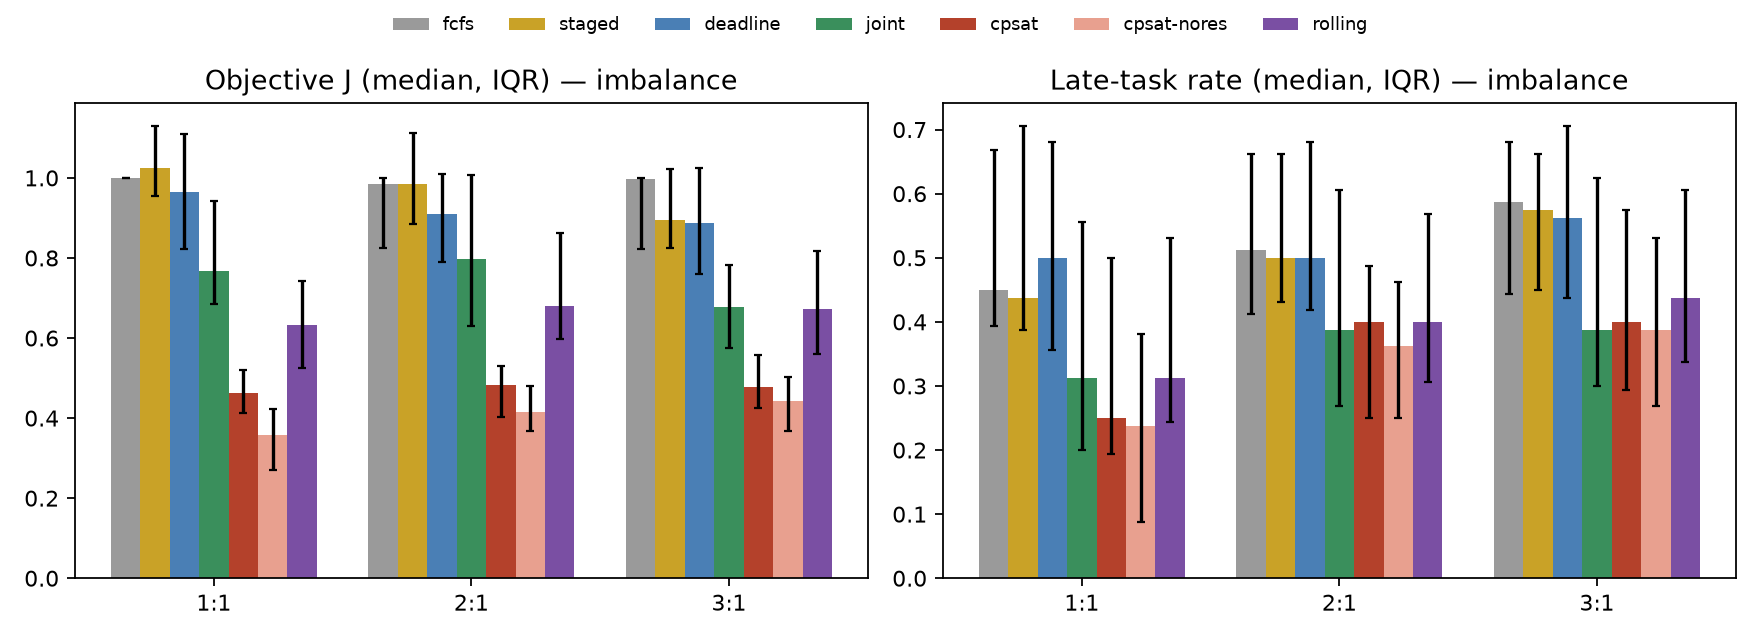
\includegraphics[width=0.92\linewidth]{imbalance.png}
\caption{充电位与区域不平衡实验（中位数，四分位距）。}
\end{figure}

\begin{figure}[H]
\centering
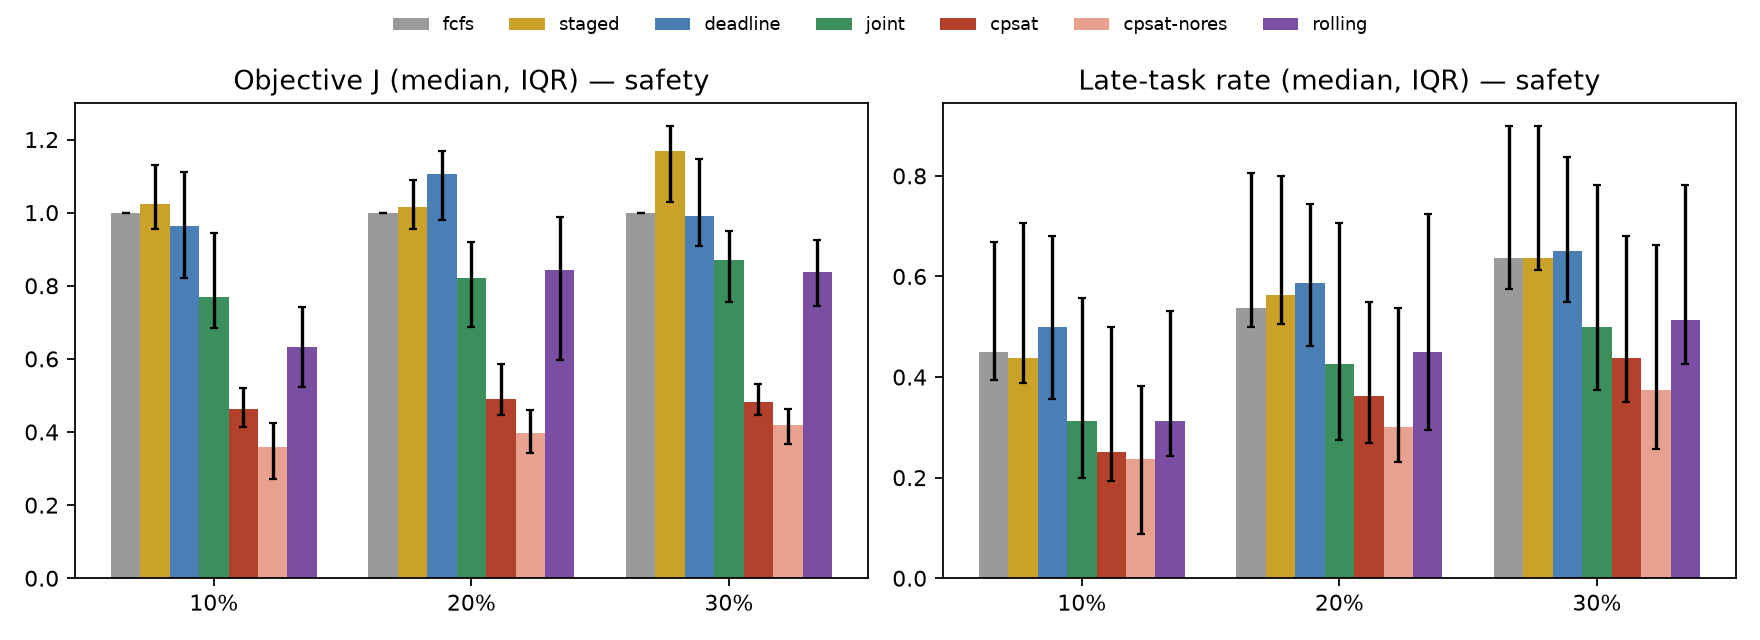
\includegraphics[width=0.92\linewidth]{safety.png}\\[2pt]
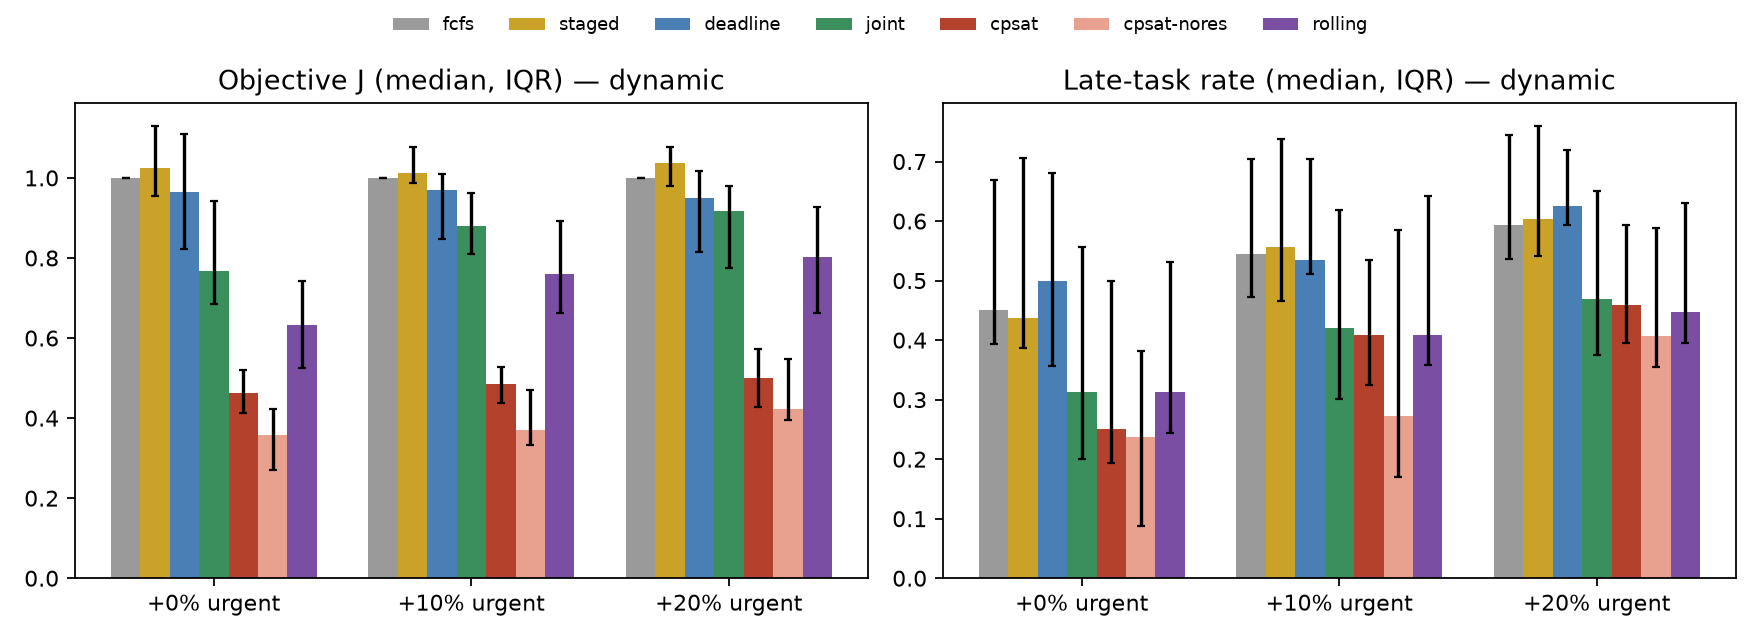
\includegraphics[width=0.92\linewidth]{dynamic.png}
\caption{安全阈值与紧急任务实验（中位数，四分位距）。}
\end{figure}

\section{讨论}

\subsection{改进从何而来？}

把 $J$ 分解为四个归一化项（基础设置，平均贡献；FCFS 每项贡献 0.25）可以看出，各方法的改进方式不同（表~\ref{tab:terms}）。

\begin{table}[H]
\centering\small
\begin{tabular}{lrrrrrr}
\toprule
策略 & $C_{\max}$ & 迟到 & 排队 & 能耗 & $J$ & $J'$\textsuperscript{c} \\
\midrule
FCFS & 0.250 & 0.250 & 0.250 & 0.250 & 1.00 & 1.00 \\
联合贪心 & 0.233 & 0.182 & 0.160 & 0.218 & 0.79 & 0.84 \\
滚动 & 0.211 & 0.157 & 0.048 & 0.219 & 0.64 & 0.78 \\
CP-SAT & 0.178 & 0.088 & 0.000 & 0.202 & 0.47 & 0.62 \\
CP-SAT 无储备 & 0.132 & 0.039 & 0.000 & 0.178 & 0.35 & 0.47 \\
\bottomrule
\end{tabular}
\caption{各归一化项对 $J$ 的平均贡献（基础设置）。\textsuperscript{c}$J' = (C_{\max} + \text{迟到} + \text{能耗})/0.75$，
即去掉排队项后对其余三项重新加权的 $J$。}
\label{tab:terms}
\end{table}

两种 CP-SAT 方法都\emph{几乎消除了排队}（CP-SAT 平均 5.6\,s，且全部来自一个种子；启发式规则在 X 处为 23--37\,s，在充电位为
0.9--1.5 千秒）。机器人仍然会等待，但等待发生在出发前最后一个站点的断电待机状态，而不是在 X 前或 H 处。在模型中，待机不耗电，
而排队会耗电并计入 $J$，因此优化器会推迟出发直到资源空闲；启发式规则则是先预约时隙再开到等待点。这在模型内是合理的，但 CP-SAT 在
$J$ 上的改进约有一半来自排队项。去掉该项后性能层级不变（表~\ref{tab:terms} 中的 $J'$），CP-SAT 仍明显最优：相对 FCFS 总迟到时间
减少 62\pct、完工时间缩短 28\pct（相对联合贪心分别为 44\pct\ 和 23\pct）。

迟到减少的一个合理的主要来源是充电：CP-SAT 的充电次数与联合贪心相近（4.2 次对 3.9 次），但它自行选择\emph{充多少}以及何时充，
而启发式规则总是以 5\pct/min 的速度充到 95\pct，每次最长 17 分钟，且常常发生在繁忙时段。部分充电在电动车辆路径问题中同样被证明有益 \cite{keskin2016}，
第~\ref{sec:case}~节的算例在单个实例上展示了这一机制。CP-SAT 同时还改变了任务分配、顺序和出发时间，
因此实验并未单独分离出这一效应；固定 95\pct\ 目标的 CP-SAT 运行才是对照实验。

\subsection{时域末端的电量储备}
\label{sec:reserve}

最初的 CP-SAT 实验不要求最后一个任务之后保留电量。优化器因此常常以接近安全阈值的电量结束，并在初始电量足够时跳过充电：
在所有 20 个任务的实例上它从未充电，在 40 个任务时充电次数只有启发式规则的一半（2.0 次对 3.9--5.4 次）。启发式规则则总是保留足以排在满队列
之后到达充电位的电量。对 CP-SAT 施加同样的储备后，40 个任务时其 $J$ 从 0.349 升至 0.468，但在 60 个任务时几乎没有影响
（中位数 $-51$\pct\ 对 $-47$\pct），因为此时机器人无论如何都必须充电。因此，在中等负载下离线 CP-SAT 表面优势中约五分之一
（65 个百分点中的 12 个）来自时域末端效应。任何把离线方法与持续运行策略比较的研究都需要明确的末端条件。

第二个较小的教训：优化器把末端电量恰好放在储备边界上，而仿真器的储备检查在前往 H 的途中还计入了在 X 前排队的耗电，因此拒绝了许多这样的计划，
使其回退到初始解（开发过程中，一次部分运行的 115 行结果中有 32 行回退，部分实例在多个实验中重复计数；这些行已被丢弃）。加入
$\delta = 0.5$\pct\ 的余量后，最终 100 个实例中没有一个回退。模型与仿真器的精确一致，恰恰在优化器逼近约束边界时最为重要。

\subsection{归一化目标函数}
\label{sec:norm}

按 FCFS 归一化达到了目的：否则按优先级加权的迟到时间（数万秒）会比其他项大两个数量级，而归一化后四项的贡献相当。代价是在 FCFS
某一项接近零的实例上结果不稳定。在一个 2:1 实例上，FCFS 只排队了 18\,s，于是排队项被除以 60\,s 的下限，联合贪心 735\,s 的排队
单独就为其 $J$ 增加了 $0.25 \times 735/60 \approx 3.06$（总计 3.7），尽管联合贪心在完工时间、迟到和能耗上都优于 FCFS。同样的效应使
20 个任务时分阶段和截止时间优先的均值大于 1（中位数为 0.96--0.97）。因此全文报告中位数和配对比较。更稳健的做法是用固定的、与实例无关的
尺度归一化（例如整个实验的均值），或用该实例上所有策略的中位数归一化。

\subsection{在线与离线}

滚动策略是唯一不知道未来任务的方法，但在基础设置下它仍优于所有预知未来任务的启发式规则（中位数 $-37$\pct\ 对联合贪心的 $-23$\pct），
并且在 20 个任务、单个充电位、2:1 区域不平衡和紧急任务设置下比联合贪心领先 8--14 个百分点。它的弱点正是滚动时域方法的典型问题：
在 20--30\pct\ 的安全阈值下，每个窗口的储备要求迫使其提前充电；在 60 个任务或 3:1 不平衡时，短视的前瞻无法绕开瓶颈，因此只与联合贪心
持平（在 20\pct\ 阈值下略落后）。它的每次重规划受确定性求解工作量约束（在 2 vCPU 机器上每次约 1\,s，一整天 40 个任务共 49\,s），
因此可以实时运行。在 OR-Tools 版本相同、单线程且墙钟上限不起作用的条件下，其调度在不同机器上逐位一致（已在两台机器上验证）；
运行时间自然不同。

\subsection{局限性}

\begin{itemize}
\item CP-SAT 结果依赖硬件（墙钟时间预算）；所有结果都在同一机型上得到。
\item 最优性间隙较大；要声称接近最优，需要更好的下界（例如按环路的松弛）。
\item 启发式规则能看到所有未来任务，这相对滚动策略对其有利，但相对离线 CP-SAT 则不然。
\item 充电模型是线性的，而实际电池在接近充满时充电变慢 \cite{montoya2017}；网络只有一个交叉口，机器人沿固定路线移动，
  不考虑运动学和一般的路径规划 \cite{stern2019}。
\end{itemize}

\section{结论}

本项目为共用一个交叉口和一个充电区的两条配送环路构建了仿真器，配有独立验证器、浏览器回放以及在相同固定种子实例上比较六种策略
（另加一个消融实验）的实验流程。在 700 次通过验证的运行中：
\begin{enumerate}
\item \textbf{联合决定任务、交叉口时隙和充电是值得的。}在基础设置下，各单一规则基线（FCFS、截止时间优先、分阶段）彼此相差不过几个百分点，
  联合贪心启发式改进约 20\pct，而在一个模型中优化全部决策的 CP-SAT 在 $J$ 上改进约 50\pct（相对 FCFS 迟到时间减少 62\pct、完工时间缩短
  28\pct）。在所有敏感性设置下，CP-SAT 保持在 $-47$\pct\ 到 $-62$\pct（中位数），联合贪心在 $-8$\pct\ 到 $-30$\pct\ 之间变化，
  而分阶段基线可能比 FCFS 差很多（单个充电位时 $+45$\pct）。
\item \textbf{充电是瓶颈。}高负载下限制队伍的是充电位而不是交叉口：对每种启发式规则，每次运行在 X 处的平均排队都不到一分钟，
  而充电排队可达数千秒。选择充多少、何时充是 CP-SAT 迟到更少的最合理解释（尚未通过实验单独分离），而把充电决策与任务分配分开
  （分阶段基线）在单个充电位时表现最差。
\item \textbf{在线再优化是可行的。}滚动 CP-SAT 在不知道未来任务的情况下，在中等负载时优于所有启发式规则，每次重规划约需一秒；
  在高负载或高安全阈值下它只与联合贪心启发式持平。
\item \textbf{公平比较需要谨慎。}要求相同的时域末端电量储备显著改变了 CP-SAT 的结果（$J$：0.35 $\to$ 0.47），而归一化目标函数必须结合
  中位数解读，因为接近零的参考项可能主导它。
\end{enumerate}

% Shared bibliography for report_en.tex and report_zh.tex (% Shared bibliography for report_en.tex and report_zh.tex (% Shared bibliography for report_en.tex and report_zh.tex (\input{references}).
\begin{thebibliography}{99}
\small\raggedright

% --- CP-SAT, constraint programming and scheduling ---------------------------------------------
\bibitem{perron2023cpsat}
L.~Perron, F.~Didier, and S.~Gay, ``The CP-SAT-LP Solver,'' in \emph{29th International
Conference on Principles and Practice of Constraint Programming (CP 2023)}, LIPIcs, vol.~280,
pp.~3:1--3:2, 2023, doi:10.4230/LIPIcs.CP.2023.3.

\bibitem{ortools}
% Google recommends this solver-specific citation for publications using CP-SAT.
L.~Perron and F.~Didier, \emph{CP-SAT}, OR-Tools version~9.15.6755, Google, 2026.
[Online]. Available: \url{https://developers.google.com/optimization/cp/cp_solver/}

\bibitem{ohrimenko2009}
O.~Ohrimenko, P.~J. Stuckey, and M.~Codish, ``Propagation via lazy clause generation,''
\emph{Constraints}, vol.~14, no.~3, pp.~357--391, 2009, doi:10.1007/s10601-008-9064-x.

\bibitem{laborie2018}
P.~Laborie, J.~Rogerie, P.~Shaw, and P.~Vil\'{\i}m, ``IBM ILOG CP optimizer for scheduling:
20+ years of scheduling with constraints at IBM/ILOG,''
\emph{Constraints}, vol.~23, no.~2, pp.~210--250, 2018, doi:10.1007/s10601-018-9281-x.

\bibitem{baptiste2001}
P.~Baptiste, C.~Le~Pape, and W.~Nuijten, \emph{Constraint-Based Scheduling: Applying Constraint
Programming to Scheduling Problems}, 1st~ed. Boston, MA: Kluwer Academic Publishers, 2001,
doi:10.1007/978-1-4615-1479-4.

\bibitem{shaw1998}
P.~Shaw, ``Using constraint programming and local search methods to solve vehicle routing
problems,'' in \emph{Principles and Practice of Constraint Programming --- CP98}, LNCS, vol.~1520,
pp.~417--431, 1998, doi:10.1007/3-540-49481-2\_30.

\bibitem{pinedo2016}
M.~L. Pinedo, \emph{Scheduling: Theory, Algorithms, and Systems}, 5th~ed. Cham: Springer, 2016,
doi:10.1007/978-3-319-26580-3.

\bibitem{liu1973}
C.~L. Liu and J.~W. Layland, ``Scheduling algorithms for multiprogramming in a hard-real-time
environment,'' \emph{J.\ ACM}, vol.~20, no.~1, pp.~46--61, 1973, doi:10.1145/321738.321743.

% --- AGV scheduling and control -----------------------------------------------------------------
\bibitem{vis2006}
I.~F.~A. Vis, ``Survey of research in the design and control of automated guided vehicle
systems,'' \emph{European Journal of Operational Research}, vol.~170, no.~3, pp.~677--709, 2006,
doi:10.1016/j.ejor.2004.09.020.

\bibitem{leanh2006}
T.~Le-Anh and M.~B.~M. De~Koster, ``A review of design and control of automated guided vehicle
systems,'' \emph{European Journal of Operational Research}, vol.~171, no.~1, pp.~1--23, 2006,
doi:10.1016/j.ejor.2005.01.036.

\bibitem{qiu2002}
L.~Qiu, W.-J. Hsu, S.-Y. Huang, and H.~Wang, ``Scheduling and routing algorithms for AGVs: a
survey,'' \emph{International Journal of Production Research}, vol.~40, no.~3, pp.~745--760,
2002, doi:10.1080/00207540110091712.

\bibitem{ganesharajah1998}
% Replaces Fazlollahtabar & Saidi-Mehrabad (2015), retracted on 2023-07-12.
T.~Ganesharajah, N.~G. Hall, and C.~Sriskandarajah, ``Design and operational issues in
AGV-served manufacturing systems,'' \emph{Annals of Operations Research}, vol.~76,
pp.~109--154, 1998, doi:10.1023/A:1018936219150.

\bibitem{deryck2020}
M.~De~Ryck, M.~Versteyhe, and F.~Debrouwere, ``Automated guided vehicle systems,
state-of-the-art control algorithms and techniques,'' \emph{Journal of Manufacturing Systems},
vol.~54, pp.~152--173, 2020, doi:10.1016/j.jmsy.2019.12.002.

\bibitem{wurman2008}
P.~R. Wurman, R.~D'Andrea, and M.~Mountz, ``Coordinating hundreds of cooperative, autonomous
vehicles in warehouses,'' \emph{AI Magazine}, vol.~29, no.~1, pp.~9--19, 2008,
doi:10.1609/aimag.v29i1.2082.

\bibitem{stern2019}
% Author order and initials follow the published PDF; the web metadata differs.
R.~Stern, N.~R. Sturtevant, A.~Felner, S.~Koenig, H.~Ma, T.~T. Walker, J.~Li,
D.~Atzmon, L.~Cohen, T.~K.~S. Kumar, E.~Boyarski, and R.~Bart\'{a}k,
``Multi-Agent Pathfinding: Definitions, Variants, and Benchmarks,'' in
\emph{Proceedings of the International Symposium on Combinatorial Search (SoCS 2019)},
vol.~10, no.~1, pp.~151--158, 2019,
doi:10.1609/socs.v10i1.18510.

\bibitem{dresner2008}
K.~Dresner and P.~Stone, ``A multiagent approach to autonomous intersection management,''
\emph{Journal of Artificial Intelligence Research}, vol.~31, pp.~591--656, 2008,
doi:10.1613/jair.2502.

% --- Battery and charging -----------------------------------------------------------------------
\bibitem{mchaney1995}
R.~McHaney, ``Modelling battery constraints in discrete event automated guided vehicle
simulations,'' \emph{International Journal of Production Research}, vol.~33, no.~11,
pp.~3023--3040, 1995, doi:10.1080/00207549508904859.

\bibitem{kabir2018}
Q.~S. Kabir and Y.~Suzuki, ``Increasing manufacturing flexibility through battery management of
automated guided vehicles,'' \emph{Computers \& Industrial Engineering}, vol.~117, pp.~225--236,
2018, doi:10.1016/j.cie.2018.01.026.

\bibitem{schneider2014}
M.~Schneider, A.~Stenger, and D.~Goeke, ``The electric vehicle-routing problem with time windows
and recharging stations,'' \emph{Transportation Science}, vol.~48, no.~4, pp.~500--520, 2014,
doi:10.1287/trsc.2013.0490.

\bibitem{keskin2016}
M.~Keskin and B.~\c{C}atay, ``Partial recharge strategies for the electric vehicle routing
problem with time windows,'' \emph{Transportation Research Part C: Emerging Technologies},
vol.~65, pp.~111--127, 2016, doi:10.1016/j.trc.2016.01.013.

\bibitem{montoya2017}
A.~Montoya, C.~Gu\'eret, J.~E. Mendoza, and J.~G. Villegas, ``The electric vehicle routing problem
with nonlinear charging function,'' \emph{Transportation Research Part B: Methodological},
vol.~103, pp.~87--110, 2017, doi:10.1016/j.trb.2017.02.004.

% --- Rolling horizon ----------------------------------------------------------------------------
\bibitem{sethi1991}
S.~Sethi and G.~Sorger, ``A theory of rolling horizon decision making,'' \emph{Annals of
Operations Research}, vol.~29, no.~1, pp.~387--415, 1991, doi:10.1007/BF02283607.

\bibitem{mayne2000}
D.~Q. Mayne, J.~B. Rawlings, C.~V. Rao, and P.~O.~M. Scokaert, ``Constrained model predictive
control: stability and optimality,'' \emph{Automatica}, vol.~36, no.~6, pp.~789--814, 2000,
doi:10.1016/S0005-1098(99)00214-9.

\end{thebibliography}
).
\begin{thebibliography}{99}
\small\raggedright

% --- CP-SAT, constraint programming and scheduling ---------------------------------------------
\bibitem{perron2023cpsat}
L.~Perron, F.~Didier, and S.~Gay, ``The CP-SAT-LP Solver,'' in \emph{29th International
Conference on Principles and Practice of Constraint Programming (CP 2023)}, LIPIcs, vol.~280,
pp.~3:1--3:2, 2023, doi:10.4230/LIPIcs.CP.2023.3.

\bibitem{ortools}
% Google recommends this solver-specific citation for publications using CP-SAT.
L.~Perron and F.~Didier, \emph{CP-SAT}, OR-Tools version~9.15.6755, Google, 2026.
[Online]. Available: \url{https://developers.google.com/optimization/cp/cp_solver/}

\bibitem{ohrimenko2009}
O.~Ohrimenko, P.~J. Stuckey, and M.~Codish, ``Propagation via lazy clause generation,''
\emph{Constraints}, vol.~14, no.~3, pp.~357--391, 2009, doi:10.1007/s10601-008-9064-x.

\bibitem{laborie2018}
P.~Laborie, J.~Rogerie, P.~Shaw, and P.~Vil\'{\i}m, ``IBM ILOG CP optimizer for scheduling:
20+ years of scheduling with constraints at IBM/ILOG,''
\emph{Constraints}, vol.~23, no.~2, pp.~210--250, 2018, doi:10.1007/s10601-018-9281-x.

\bibitem{baptiste2001}
P.~Baptiste, C.~Le~Pape, and W.~Nuijten, \emph{Constraint-Based Scheduling: Applying Constraint
Programming to Scheduling Problems}, 1st~ed. Boston, MA: Kluwer Academic Publishers, 2001,
doi:10.1007/978-1-4615-1479-4.

\bibitem{shaw1998}
P.~Shaw, ``Using constraint programming and local search methods to solve vehicle routing
problems,'' in \emph{Principles and Practice of Constraint Programming --- CP98}, LNCS, vol.~1520,
pp.~417--431, 1998, doi:10.1007/3-540-49481-2\_30.

\bibitem{pinedo2016}
M.~L. Pinedo, \emph{Scheduling: Theory, Algorithms, and Systems}, 5th~ed. Cham: Springer, 2016,
doi:10.1007/978-3-319-26580-3.

\bibitem{liu1973}
C.~L. Liu and J.~W. Layland, ``Scheduling algorithms for multiprogramming in a hard-real-time
environment,'' \emph{J.\ ACM}, vol.~20, no.~1, pp.~46--61, 1973, doi:10.1145/321738.321743.

% --- AGV scheduling and control -----------------------------------------------------------------
\bibitem{vis2006}
I.~F.~A. Vis, ``Survey of research in the design and control of automated guided vehicle
systems,'' \emph{European Journal of Operational Research}, vol.~170, no.~3, pp.~677--709, 2006,
doi:10.1016/j.ejor.2004.09.020.

\bibitem{leanh2006}
T.~Le-Anh and M.~B.~M. De~Koster, ``A review of design and control of automated guided vehicle
systems,'' \emph{European Journal of Operational Research}, vol.~171, no.~1, pp.~1--23, 2006,
doi:10.1016/j.ejor.2005.01.036.

\bibitem{qiu2002}
L.~Qiu, W.-J. Hsu, S.-Y. Huang, and H.~Wang, ``Scheduling and routing algorithms for AGVs: a
survey,'' \emph{International Journal of Production Research}, vol.~40, no.~3, pp.~745--760,
2002, doi:10.1080/00207540110091712.

\bibitem{ganesharajah1998}
% Replaces Fazlollahtabar & Saidi-Mehrabad (2015), retracted on 2023-07-12.
T.~Ganesharajah, N.~G. Hall, and C.~Sriskandarajah, ``Design and operational issues in
AGV-served manufacturing systems,'' \emph{Annals of Operations Research}, vol.~76,
pp.~109--154, 1998, doi:10.1023/A:1018936219150.

\bibitem{deryck2020}
M.~De~Ryck, M.~Versteyhe, and F.~Debrouwere, ``Automated guided vehicle systems,
state-of-the-art control algorithms and techniques,'' \emph{Journal of Manufacturing Systems},
vol.~54, pp.~152--173, 2020, doi:10.1016/j.jmsy.2019.12.002.

\bibitem{wurman2008}
P.~R. Wurman, R.~D'Andrea, and M.~Mountz, ``Coordinating hundreds of cooperative, autonomous
vehicles in warehouses,'' \emph{AI Magazine}, vol.~29, no.~1, pp.~9--19, 2008,
doi:10.1609/aimag.v29i1.2082.

\bibitem{stern2019}
% Author order and initials follow the published PDF; the web metadata differs.
R.~Stern, N.~R. Sturtevant, A.~Felner, S.~Koenig, H.~Ma, T.~T. Walker, J.~Li,
D.~Atzmon, L.~Cohen, T.~K.~S. Kumar, E.~Boyarski, and R.~Bart\'{a}k,
``Multi-Agent Pathfinding: Definitions, Variants, and Benchmarks,'' in
\emph{Proceedings of the International Symposium on Combinatorial Search (SoCS 2019)},
vol.~10, no.~1, pp.~151--158, 2019,
doi:10.1609/socs.v10i1.18510.

\bibitem{dresner2008}
K.~Dresner and P.~Stone, ``A multiagent approach to autonomous intersection management,''
\emph{Journal of Artificial Intelligence Research}, vol.~31, pp.~591--656, 2008,
doi:10.1613/jair.2502.

% --- Battery and charging -----------------------------------------------------------------------
\bibitem{mchaney1995}
R.~McHaney, ``Modelling battery constraints in discrete event automated guided vehicle
simulations,'' \emph{International Journal of Production Research}, vol.~33, no.~11,
pp.~3023--3040, 1995, doi:10.1080/00207549508904859.

\bibitem{kabir2018}
Q.~S. Kabir and Y.~Suzuki, ``Increasing manufacturing flexibility through battery management of
automated guided vehicles,'' \emph{Computers \& Industrial Engineering}, vol.~117, pp.~225--236,
2018, doi:10.1016/j.cie.2018.01.026.

\bibitem{schneider2014}
M.~Schneider, A.~Stenger, and D.~Goeke, ``The electric vehicle-routing problem with time windows
and recharging stations,'' \emph{Transportation Science}, vol.~48, no.~4, pp.~500--520, 2014,
doi:10.1287/trsc.2013.0490.

\bibitem{keskin2016}
M.~Keskin and B.~\c{C}atay, ``Partial recharge strategies for the electric vehicle routing
problem with time windows,'' \emph{Transportation Research Part C: Emerging Technologies},
vol.~65, pp.~111--127, 2016, doi:10.1016/j.trc.2016.01.013.

\bibitem{montoya2017}
A.~Montoya, C.~Gu\'eret, J.~E. Mendoza, and J.~G. Villegas, ``The electric vehicle routing problem
with nonlinear charging function,'' \emph{Transportation Research Part B: Methodological},
vol.~103, pp.~87--110, 2017, doi:10.1016/j.trb.2017.02.004.

% --- Rolling horizon ----------------------------------------------------------------------------
\bibitem{sethi1991}
S.~Sethi and G.~Sorger, ``A theory of rolling horizon decision making,'' \emph{Annals of
Operations Research}, vol.~29, no.~1, pp.~387--415, 1991, doi:10.1007/BF02283607.

\bibitem{mayne2000}
D.~Q. Mayne, J.~B. Rawlings, C.~V. Rao, and P.~O.~M. Scokaert, ``Constrained model predictive
control: stability and optimality,'' \emph{Automatica}, vol.~36, no.~6, pp.~789--814, 2000,
doi:10.1016/S0005-1098(99)00214-9.

\end{thebibliography}
).
\begin{thebibliography}{99}
\small\raggedright

% --- CP-SAT, constraint programming and scheduling ---------------------------------------------
\bibitem{perron2023cpsat}
L.~Perron, F.~Didier, and S.~Gay, ``The CP-SAT-LP Solver,'' in \emph{29th International
Conference on Principles and Practice of Constraint Programming (CP 2023)}, LIPIcs, vol.~280,
pp.~3:1--3:2, 2023, doi:10.4230/LIPIcs.CP.2023.3.

\bibitem{ortools}
% Google recommends this solver-specific citation for publications using CP-SAT.
L.~Perron and F.~Didier, \emph{CP-SAT}, OR-Tools version~9.15.6755, Google, 2026.
[Online]. Available: \url{https://developers.google.com/optimization/cp/cp_solver/}

\bibitem{ohrimenko2009}
O.~Ohrimenko, P.~J. Stuckey, and M.~Codish, ``Propagation via lazy clause generation,''
\emph{Constraints}, vol.~14, no.~3, pp.~357--391, 2009, doi:10.1007/s10601-008-9064-x.

\bibitem{laborie2018}
P.~Laborie, J.~Rogerie, P.~Shaw, and P.~Vil\'{\i}m, ``IBM ILOG CP optimizer for scheduling:
20+ years of scheduling with constraints at IBM/ILOG,''
\emph{Constraints}, vol.~23, no.~2, pp.~210--250, 2018, doi:10.1007/s10601-018-9281-x.

\bibitem{baptiste2001}
P.~Baptiste, C.~Le~Pape, and W.~Nuijten, \emph{Constraint-Based Scheduling: Applying Constraint
Programming to Scheduling Problems}, 1st~ed. Boston, MA: Kluwer Academic Publishers, 2001,
doi:10.1007/978-1-4615-1479-4.

\bibitem{shaw1998}
P.~Shaw, ``Using constraint programming and local search methods to solve vehicle routing
problems,'' in \emph{Principles and Practice of Constraint Programming --- CP98}, LNCS, vol.~1520,
pp.~417--431, 1998, doi:10.1007/3-540-49481-2\_30.

\bibitem{pinedo2016}
M.~L. Pinedo, \emph{Scheduling: Theory, Algorithms, and Systems}, 5th~ed. Cham: Springer, 2016,
doi:10.1007/978-3-319-26580-3.

\bibitem{liu1973}
C.~L. Liu and J.~W. Layland, ``Scheduling algorithms for multiprogramming in a hard-real-time
environment,'' \emph{J.\ ACM}, vol.~20, no.~1, pp.~46--61, 1973, doi:10.1145/321738.321743.

% --- AGV scheduling and control -----------------------------------------------------------------
\bibitem{vis2006}
I.~F.~A. Vis, ``Survey of research in the design and control of automated guided vehicle
systems,'' \emph{European Journal of Operational Research}, vol.~170, no.~3, pp.~677--709, 2006,
doi:10.1016/j.ejor.2004.09.020.

\bibitem{leanh2006}
T.~Le-Anh and M.~B.~M. De~Koster, ``A review of design and control of automated guided vehicle
systems,'' \emph{European Journal of Operational Research}, vol.~171, no.~1, pp.~1--23, 2006,
doi:10.1016/j.ejor.2005.01.036.

\bibitem{qiu2002}
L.~Qiu, W.-J. Hsu, S.-Y. Huang, and H.~Wang, ``Scheduling and routing algorithms for AGVs: a
survey,'' \emph{International Journal of Production Research}, vol.~40, no.~3, pp.~745--760,
2002, doi:10.1080/00207540110091712.

\bibitem{ganesharajah1998}
% Replaces Fazlollahtabar & Saidi-Mehrabad (2015), retracted on 2023-07-12.
T.~Ganesharajah, N.~G. Hall, and C.~Sriskandarajah, ``Design and operational issues in
AGV-served manufacturing systems,'' \emph{Annals of Operations Research}, vol.~76,
pp.~109--154, 1998, doi:10.1023/A:1018936219150.

\bibitem{deryck2020}
M.~De~Ryck, M.~Versteyhe, and F.~Debrouwere, ``Automated guided vehicle systems,
state-of-the-art control algorithms and techniques,'' \emph{Journal of Manufacturing Systems},
vol.~54, pp.~152--173, 2020, doi:10.1016/j.jmsy.2019.12.002.

\bibitem{wurman2008}
P.~R. Wurman, R.~D'Andrea, and M.~Mountz, ``Coordinating hundreds of cooperative, autonomous
vehicles in warehouses,'' \emph{AI Magazine}, vol.~29, no.~1, pp.~9--19, 2008,
doi:10.1609/aimag.v29i1.2082.

\bibitem{stern2019}
% Author order and initials follow the published PDF; the web metadata differs.
R.~Stern, N.~R. Sturtevant, A.~Felner, S.~Koenig, H.~Ma, T.~T. Walker, J.~Li,
D.~Atzmon, L.~Cohen, T.~K.~S. Kumar, E.~Boyarski, and R.~Bart\'{a}k,
``Multi-Agent Pathfinding: Definitions, Variants, and Benchmarks,'' in
\emph{Proceedings of the International Symposium on Combinatorial Search (SoCS 2019)},
vol.~10, no.~1, pp.~151--158, 2019,
doi:10.1609/socs.v10i1.18510.

\bibitem{dresner2008}
K.~Dresner and P.~Stone, ``A multiagent approach to autonomous intersection management,''
\emph{Journal of Artificial Intelligence Research}, vol.~31, pp.~591--656, 2008,
doi:10.1613/jair.2502.

% --- Battery and charging -----------------------------------------------------------------------
\bibitem{mchaney1995}
R.~McHaney, ``Modelling battery constraints in discrete event automated guided vehicle
simulations,'' \emph{International Journal of Production Research}, vol.~33, no.~11,
pp.~3023--3040, 1995, doi:10.1080/00207549508904859.

\bibitem{kabir2018}
Q.~S. Kabir and Y.~Suzuki, ``Increasing manufacturing flexibility through battery management of
automated guided vehicles,'' \emph{Computers \& Industrial Engineering}, vol.~117, pp.~225--236,
2018, doi:10.1016/j.cie.2018.01.026.

\bibitem{schneider2014}
M.~Schneider, A.~Stenger, and D.~Goeke, ``The electric vehicle-routing problem with time windows
and recharging stations,'' \emph{Transportation Science}, vol.~48, no.~4, pp.~500--520, 2014,
doi:10.1287/trsc.2013.0490.

\bibitem{keskin2016}
M.~Keskin and B.~\c{C}atay, ``Partial recharge strategies for the electric vehicle routing
problem with time windows,'' \emph{Transportation Research Part C: Emerging Technologies},
vol.~65, pp.~111--127, 2016, doi:10.1016/j.trc.2016.01.013.

\bibitem{montoya2017}
A.~Montoya, C.~Gu\'eret, J.~E. Mendoza, and J.~G. Villegas, ``The electric vehicle routing problem
with nonlinear charging function,'' \emph{Transportation Research Part B: Methodological},
vol.~103, pp.~87--110, 2017, doi:10.1016/j.trb.2017.02.004.

% --- Rolling horizon ----------------------------------------------------------------------------
\bibitem{sethi1991}
S.~Sethi and G.~Sorger, ``A theory of rolling horizon decision making,'' \emph{Annals of
Operations Research}, vol.~29, no.~1, pp.~387--415, 1991, doi:10.1007/BF02283607.

\bibitem{mayne2000}
D.~Q. Mayne, J.~B. Rawlings, C.~V. Rao, and P.~O.~M. Scokaert, ``Constrained model predictive
control: stability and optimality,'' \emph{Automatica}, vol.~36, no.~6, pp.~789--814, 2000,
doi:10.1016/S0005-1098(99)00214-9.

\end{thebibliography}


\end{document}
